%%%%%%%%%%%%%%%%%%%%%%%%%%%%%%%%%%%%%%%%%%%%%%%%%%%%%%%%%%%%%%%%%%%%%
%
% Complete documentation on the extended LaTeX markup used for Insight
% documentation is available in ``Documenting Insight'', that is part
% of the standard documentation for Insight.  It may be found online
% at:
%
%                    http://www.itk.org
%
%%%%%%%%%%%%%%%%%%%%%%%%%%%%%%%%%%%%%%%%%%%%%%%%%%%%%%%%%%%%%%%%%%%%%

\documentclass{InsightSoftwareGuide}


\usepackage[dvips]{graphicx}
\usepackage{times,lscape,url}
%\usepackage{mdwtab}


%%% \usepackage[latin1]{inputenc}
%%% \selectlanguage{french}
% Configuration pour les accents francais pour l'OTB
\usepackage[latin1]{inputenc}
%\usepackage[french]{babel}
\usepackage{tikz}

\usepackage{color}

\definecolor{listcomment}{rgb}{0.0,0.5,0.0}
\definecolor{listkeyword}{rgb}{0.0,0.0,0.5}
\definecolor{listnumbers}{gray}{0.65}
\definecolor{listlightgray}{gray}{0.955}
\definecolor{listwhite}{gray}{1.0}

\usepackage{minted}
\newminted{cpp}{fontsize=\small}
\newminted{cmake}{fontsize=\small}
\newminted{bat}{fontsize=\small}

\usepackage{mdframed}
\BeforeBeginEnvironment{cppcode}{\begin{mdframed}[leftline=false,rightline=false,backgroundcolor=listlightgray]}
\AfterEndEnvironment{cppcode}{\end{mdframed}}

\newif\ifitkFullVersion
\itkFullVersiontrue
%\itkFullVersionfalse

\newif\ifitkPrintedVersion
\itkPrintedVersiontrue
%\itkPrintedVersionfalse

\usepackage{multicol}

%%%%%%%%%%%%%%%%%%%%%%%%%%%%%%%%%%%%%%%%%%%%%%%%%%%%%%%%%%%%%%%%%%
%
%  hyperref should be the last package to be loaded.
%
%%%%%%%%%%%%%%%%%%%%%%%%%%%%%%%%%%%%%%%%%%%%%%%%%%%%%%%%%%%%%%%%%%
\ifitkPrintedVersion
\usepackage[dvips,
pdftitle={OTB Software Guide},
pdfauthor={CNES},
pdfsubject={Remote Sensing, Orfeo, Pleiades, Cosmo Skymed},
pdfkeywords={Image processing, Remote sensing, Guide},
pdfpagemode={UseOutlines},
bookmarks,bookmarksopen,
pdfstartview={FitH},
backref,
colorlinks,linkcolor={black},citecolor={black},urlcolor={black},
]{hyperref}
\else
\usepackage[dvips,
pdftitle={OTB Software Guide},
pdfauthor={CNES},
pdfsubject={Remote Sensing, Orfeo, Pleiades, Cosmo Skymed},
pdfkeywords={Image processing, Remote sensing, Guide},
pdfpagemode={UseOutlines},
bookmarks,bookmarksopen,
pdfstartview={FitH},
backref,
colorlinks,linkcolor={blue},citecolor={blue},urlcolor={blue},
]{hyperref}
\fi

\usepackage{amsmath,amssymb,amsfonts}
\usepackage{bbm}
%%%%%%%%%%%%%%%%%%%%%%%%%%%%%%%%%%%%%%%%%%%%%%%%%%%%%%%%%%%%%%%%%%%
%
%
%   Load configuration parameters prepared by CMake
%
%
%%%%%%%%%%%%%%%%%%%%%%%%%%%%%%%%%%%%%%%%%%%%%%%%%%%%%%%%%%%%%%%%%%%

\input{SoftwareGuideConfiguration.tex}

\def\logoCNES{CNES_nom.eps}

\newtheorem{algo}{Algorithm}
\newtheorem{defin}{Definition}
%%%%%%%%%%%%%%%%%%%%%%%%%%%%%%%%%%%%%%%%%%%%%%%%%%%%%%%%%%%%%%%%%%%
%
%
%           The Insight Toolkit Software Guide
%
%
%%%%%%%%%%%%%%%%%%%%%%%%%%%%%%%%%%%%%%%%%%%%%%%%%%%%%%%%%%%%%%%%%%%

\title{The ORFEO Tool Box Software Guide\\ Updated
  for OTB-\otbversion}

\author{OTB Development Team}

\authoraddress{
  \url{http://www.orfeo-toolbox.org}\\
  e-mail: \email{otb@cnes.fr}
}

\date{\today}


% actually write the .idx file
\makeindex

\setcounter{tocdepth}{3}



%%%%%%%%%%%%%%%%%%%%%%%%%%%%%%%%%%%%%%%%%%%%%%%%%%%%%%%%%%%%%%%%%%%
%
%           Begin Document
%
%%%%%%%%%%%%%%%%%%%%%%%%%%%%%%%%%%%%%%%%%%%%%%%%%%%%%%%%%%%%%%%%%%%

\begin{document}

\ifitkPrintedVersion
%% \input{PrintedPreamble.tex}
\fi

\maketitle

\frontmatter

\hyperbaseurl{http://www.orfeo-toolbox.org}


%%%%%%%%%%%%%%%%%%%%%%%%%%%%%%%%%%%%%%%%%%
%
%  Page with OTB logo
%
%%%%%%%%%%%%%%%%%%%%%%%%%%%%%%%%%%%%%%%%%%
\cleardoublepage

\begin{minipage}[t][10cm][b]{\textwidth}
\center
\includegraphics[width=0.5\textwidth]{logoVectoriel.eps}
\large
\begin{center}
\emph{The ORFEO Toolbox is not a black box.}\\
\end{center}
\hspace{8cm} Ch.D.
\normalsize
\end{minipage}



%%%%%%%%%%%%%%%%%%%%%%%%%%%%%%%%%%%%%%%%%%%%%%
%
% remove headings from the following material
\pagestyle{plain}
%
%%%%%%%%%%%%%%%%%%%%%%%%%%%%%%%%%%%%%%%%%%%%%%



%%\ifitkPrintedVersion
%% \input{Cover.tex}
%%\fi

\input{Abstract.tex}




%%%%%%%%%%%%%%%%%%%%%%%%%%%%%%%%%%%%%%%%%%%%%%%%%%%%%%%%%
%
% Insert Table of Contents; List of Figures and Tables
%
%%%%%%%%%%%%%%%%%%%%%%%%%%%%%%%%%%%%%%%%%%%%%%%%%%%%%%%%%


%%%%%%%%%%%%%%%%%%%%%%%%%%%%%%%%%%%%%%%%%%%%%%
%
% enable headings from the following material
\pagestyle{normal}
%
%%%%%%%%%%%%%%%%%%%%%%%%%%%%%%%%%%%%%%%%%%%%%%
\small
\tableofcontents
\listoffigures
\listoftables
\normalsize




%%%%%%%%%%%%%%%%%%%%%%%%%%%%%%%%%%%%%%%%%
%
% Begin technical content
%
%%%%%%%%%%%%%%%%%%%%%%%%%%%%%%%%%%%%%%%%%

\mainmatter

\part{Introduction}\label{part:introduction}

\chapter{Welcome}
\label{chapter:Welcome}

Welcome to the \emph{ORFEO ToolBox (OTB) Software Guide}.

This document presents the essential concepts used in OTB. It will
guide you through the road of learning and using OTB. The Doxygen
documentation for the OTB application programming interface is
available on line at \url{https://www.orfeo-toolbox.org/doxygen}.

\section{Organization}
\label{sec:Organization}

This software guide is divided into several parts, each of which is further
divided into several chapters. Part~\ref{part:introduction} is a general
introduction to OTB,
with---in the next chapter---a description of how to install the ORFEO
Toolbox on your computer. Part~\ref{part:introduction} also
introduces basic system concepts such as an overview of the system
architecture, and how to build applications in the C++ programming
language. Part \ref{part:tutorials} is a short guide with gradual difficulty to
get you start programming with OTB. Part~\ref{part:userguide} describes the
system from the user point of view. Dozens
of examples are used to illustrate important system features.
Part~\ref{part:developerguide}  is for
the OTB developer. It explains how to create your own classes and extend
the system.%, and interface to windowing and GUI systems.

\section{How to Learn OTB}
\label{sec:HowToLearnOTB}

There are two broad categories of users of OTB. First are class
developers, those who create classes in C++. The second, users, employ
existing C++ classes to build applications. Class developers must be
proficient in C++, and if they are extending or modifying OTB, they
must also be familiar with OTB's internal structures and design
(material covered in Part~\ref{part:developerguide}).

The key to learning how to use OTB is to become familiar with its
palette of objects and the ways of combining them. We recommend that you learn
the system by studying the
examples and then, if you are a class developer, study the source
code. Start by the first few tutorials in Part~\ref{part:tutorials} to get
familiar with the build process and the general program organization, follow by
reading Chapter \ref{chapter:SystemOverview}, which provides an overview of some
of the key concepts in the system, and then review the examples in
Part~\ref{part:userguide}. You may also wish to compile and run the dozens of
examples
distributed with the source code found in the directory
\code{OTB/Examples}. (Please see the file
\code{OTB/Examples/README.txt} for a description of the examples
contained in the various subdirectories.) There are also several
hundreds of tests found in the source distribution in
\code{OTB/Testing/Code}, most of which are minimally documented
testing code. However, they may be useful to see how classes are used
together in OTB, especially since they are designed to exercise as
much of the functionality of each class as possible.

\section{Software Organization}
\label{sec:SoftwareOrganization}

The following sections describe the directory contents, summarize the
software functionality in each directory, and locate the documentation and
data.

\subsection{Obtaining the Software}
\label{sec:ObtainingTheSoftware}

Periodic releases of the software are available on the OTB Website. These
official releases are available a few times a year and announced on the ORFEO
Web pages and mailing lists.

This software guide assumes that you are working with the latest official OTB
release (available on the OTB Web site). %If you are a new user,
%we highly recommend that you use the released version of the software.


OTB can be downloaded without cost from the following web site:
\begin{center}
  \url{http://www.orfeo-toolbox.org/}
\end{center}
In order to track the kind of applications for which OTB is being used, you
will be asked to complete a form prior to downloading the software.
The information you provide in this form will help developers to get a better
idea of the interests and skills of the toolkit users.

Once you fill out this form you will have access to the download
page. This page can be book marked to facilitate subsequent visits to
the download site without having to complete any form again.

 Then choose the tarball that better fits your system. The options
are \code{.zip} and \code{.tgz} files.  The first type is better suited for
MS-Windows while the second one is the preferred format for UNIX systems.

Once you unzip or untar the file, a directory called \code{OTB} will be
created in your disk and you will be ready for starting the configuration
process described in Section \ref{chapter:Installation}.


There are two other ways of getting the OTB source code:
\begin{itemize}
\item Clone the current release with \href{https://git-scm.com/}{Git} from the
  \href{https://gitlab.orfeo-toolbox.org/orfeotoolbox/otb.git}{OTB git server}, (master branch)
\item Clone the latest revision with \href{https://git-scm.com/}{Git} from the
  \href{https://gitlab.orfeo-toolbox.org/orfeotoolbox/otb.git}{OTB git server} (develop branch).
\end{itemize}

These last two options need a proper \href{https://git-scm.com/}{Git} installation. To get source code from Git, do:
\begin{verbatim}
git clone https://gitlab.orfeo-toolbox.org/orfeotoolbox/otb.git
\end{verbatim}

Using Git, you can easily navigate through the different versions. The master
branch contains the latest stable version:
\begin{verbatim}
git checkout master
\end{verbatim}
Specific versions are availables with tags:
\begin{verbatim}
git checkout 5.2.0
\end{verbatim}
Finally, this brings you to the latest development version:
\begin{verbatim}
git checkout develop
\end{verbatim}

There is also a mirror of OTB official repository on \href{https://github.com/orfeotoolbox/OTB}{GitHub}.
You can find more information on the OTB git workflow in the \href{http://wiki.orfeo-toolbox.org/index.php/Git}{wiki}.

\subsection{Directory Structure}
\label{sec:DirectoryStructure}

To begin your OTB odyssey, you will first need to know something about OTB's
software organization and directory structure. It is helpful to know enough to
navigate through the code base to find examples, code, and documentation.

The \code{OTB} contains the following subdirectories:
\begin{itemize}
        \item \code{OTB/Modules}---the heart of the software; the location
        of the majority of the source code.
        \item \code{OTB/CMake}---internal files used during the
        configuration process.
        \item \code{OTB/Copyright}---the copyright information of OTB
        and all the dependencies included in the OTB source tree.
        \item \code{OTB/Examples}---a suite of simple, well-documented
        examples used by this guide and to illustrate important
        OTB concepts.
        \item \code{OTB/Superbuild}---CMake scripts to automatically download, patch, build and install important
        dependencies of OTB (ITK, OSSIM, GDAL to name a few).
        \item \code{OTB/Utilities}---small programs used for the maintenance of OTB.
\end{itemize}


OTB is organized into different modules, each one covering different part of image processing.
It is therefore important to understand the source code directory structure---found in \code{OTB/Modules}---.
\begin{itemize}
  \item \code{OTB/Modules/Adapters}---Adapters for Boost, Curl, Gdal and Ossim.
  \item \code{OTB/Modules/Applications}---a set of applications modules that can be launched in different ways
    (command-line, graphical interface, Python/Java), refer to the OTB Cookbook for more information.
  \item \code{OTB/Modules/Core}---core classes, macro definitions,
  typedefs, and other software constructs central to OTB.
  \item \code{OTB/Modules/Detection}---detection of clouds, roads.
  \item \code{OTB/Modules/Feature}---various local descriptors and features.
  \item \code{OTB/Modules/Filtering}---basic image processing filters.
  \item \code{OTB/Modules/Fusion}---image fusion algorithms, as for
  instance, pansharpening.
  \item \code{OTB/Modules/Hyperspectral}---hyperspectral images analysis.
  \item \code{OTB/Modules/IO}---classes that support the reading
  and writing of data.
  \item \code{OTB/Modules/Learning}---several functionalities for
	supervised learning and classification.
  \item \code{OTB/Modules/OBIA}---Object Based Image Analysis filters
	and data structures.
  \item \code{OTB/Modules/Radiometry}---classes allowing to compute
  vegetation indices and radiometric corrections.
  \item \code{OTB/Modules/Registration}---classes for registration of images or other data structures to each other.
  \item \code{OTB/Modules/Remote}---Functions to fetch remote modules.
  \item \code{OTB/Modules/Segmentation}---several functionalities for image segmentation.
  \item \code{OTB/Modules/ThirdParty}---Modules that import OTB's dependencies.
  \item \code{OTB/Modules/Wrappers}---Applications wrappers with several access points (command-line, QT Gui, SWIG\ldots).
\end{itemize}


See also chapter \ref{chapter:newModules} for more information about how to write modules.

\subsection{Documentation}
\label{sec:Documentation}

Besides this text, there are other documentation resources that you should be
aware of.
\begin{description}
        \item[Doxygen Documentation.] The Doxygen documentation is an
        essential resource when working with OTB. These extensive Web
        pages describe in detail every class and method in the
        system. The documentation also contains inheritance and
        collaboration diagrams, listing of event invocations, and data
        members. The documentation is heavily hyper-linked to other
        classes and to the source code. The Doxygen documentation is
        available on-line at
        \url{http://www.orfeo-toolbox.org/doxygen/}.

	\item[Header Files.] Each OTB class is implemented with a .h and
        .cxx/.hxx file (.hxx file for templated classes). All methods
        found in the .h header files are documented and provide a quick way
        to find documentation for a particular method. (Indeed, Doxygen uses
        the header documentation to produces its output.)
\end{description}

\subsection{Data}
\label{sec:Data}

The OTB Toolkit was designed to support the ORFEO Acompaniment Program
and its associated data. This data is available at
\url{http://smsc.cnes.fr/PLEIADES/index.htm}.



\section{The OTB Community and Support}
\label{sec:AdditionalResources}

\subsection{Join the Mailing List}
\label{sec:JoinMailList}

\index{OTB!mailing list}
\index{mailing list}

It is strongly recommended that you join the users mailing list. This is one
of the primary resources for guidance and help regarding the use of the
toolkit. You can subscribe to the users list online at

\begin{center}
\url{http://groups.google.com/group/otb-users}
\end{center}

The otb-users mailing list is also the best mechanism for expressing your
opinions about the toolbox and to let developers know about features that you
find useful, desirable or even unnecessary. OTB developers are committed to
creating a self-sustaining open-source OTB community. Feedback from users is
fundamental to achieving this goal.

\subsection{Community}
OTB was created from its inception as a collaborative, community
effort. Research, teaching, and commercial uses of the toolkit are
expected. If you would like to participate in the community, there are a
number of possibilities.

\begin{itemize}
       \item Users may actively report bugs, defects in the system API,
       and/or submit feature requests. Currently the best way to do this is
       through the OTB users mailing list.

       \item Developers may contribute classes or improve existing
       classes. If you are a developer, you may request permission to join
       the OTB developers mailing list. Please do so by sending email to
       otb ``at'' cnes.fr. To become a developer you need to
       demonstrate both a level of competence as well as
       trustworthiness. You may wish to begin by submitting fixes to the OTB
       users mailing list.

       \item Research partnerships with members of the ORFEO
       Acompaniment Program are encouraged. CNES will encourage the use of
       OTB in proposed work and research projects.

%%        \item For those developing commercial applications with OTB,
%%        support and consulting are available from Kitware at
%%        \url{http://www.kitware.com}. Kitware also offers short OTB courses
%%        either at a site of your choice or periodically at Kitware.

       \item Educators may wish to use OTB in courses. Materials are being
       developed for this purpose, e.g., a one-day, conference course and
       semester-long graduate courses. Watch the OTB web pages or check in
       the \code{OTB-Documents/CourseWare} directory for more information.
\end{itemize}

Orfeo ToolBox is currently in the incubation stage of being part of the
OSGeo\footnote{http://www.osgeo.org/} foundation.Within the ORFEO ToolBox
community we act respectfully toward others in line with the OSGeo Code of
Conduct\footnote{http://www.osgeo.org/code\_of\_conduct}.


\section{A Brief History of OTB}
\label{sec:History}

\index{OTB!history}


Beside the Pleiades (PHR) and Cosmo-Skymed (CSK) systems developments forming
ORFEO, the dual and bilateral system (France - Italy) for Earth Observation, the
ORFEO Accompaniment Program was set up, to prepare, accompany and promote the
use and the exploitation of the images derived from these sensors.

The creation of a preparatory
program\footnote{http://smsc.cnes.fr/PLEIADES/A\_prog\_accomp.htm} is needed
because of :
\begin{itemize}
\item the new capabilities and performances of the ORFEO systems (optical and
radar high resolution, access capability, data quality, possibility to acquire
simultaneously in optic and radar),
\item the implied need of new methodological developments : new processing
methods, or adaptation of existing methods,
\item the need to realize those new developments in very close
  cooperation with the final users for better integration of new products in
their systems.

\end{itemize}

This program was initiated by CNES mid-2003 and will last until 2010 at least
It consists in two parts, between which it is necessary to keep a strong
interaction :
\begin{itemize}
\item A Thematic part
\item A Methodological part.
\end{itemize}

The Thematic part covers a large range of applications (civil and
defence ones), and aims at specifying and validating value added
products and services required by end users. This part includes
consideration about products integration in the operational systems or
processing lines. It also includes a careful thought on intermediary
structures to be developed to help non-autonomous users. Lastly, this part aims
at raising future users awareness, through practical demonstrations and
validations.

The Methodological part objective is the definition and the
development of tools for the operational exploitation of the future
submetric optic and radar images (tridimensional aspects, change
detection, texture analysis, pattern matching, optic radar
complementarities). It is mainly based on R\&D studies and doctorate
and post-doctorate research.

In this context, CNES\footnote{http://www.cnes.fr} decided to develop
the \emph{ORFEO ToolBox} (OTB), a set of algorithms encapsulated in a
software library. The goals of the OTB is to capitalize a methological
\textit{savoir faire} in order to adopt an incremental development
approach aiming to efficiently exploit the results obtained in the
frame of methodological R\&D studies.

All the developments are based on FLOSS (Free/Libre Open Source
Software) or existing CNES developments.

OTB is implemented in C++ and is mainly based on
ITK\footnote{http://www.itk.org} (Insight Toolkit):
\begin{itemize}
  \item ITK is used as the core element of OTB
  \item OTB classes inherit from ITK classes
  \item The software development procedure of OTB is strongly inspired
  from ITK's (Extreme Programming, test-based coding, Generic
  Programming, etc.)
  \item The documentation production procedure is the same as for ITK
  \item Several chapters of the Software Guide are literally copied
  from ITK's Software Guide (with permission).
  \item Many examples are taken from ITK.
\end{itemize}

\subsection{ITK's history}

In 1999 the US National Library of Medicine of the National Institutes of
Health awarded six three-year contracts to develop an open-source
registration and segmentation toolkit, that eventually came to be known as
the Insight Toolkit (ITK) and formed the basis of the Insight Software
Consortium. ITK's NIH/NLM Project Manager was Dr. Terry Yoo, who coordinated the
six prime contractors composing the Insight consortium. These consortium
members included three commercial partners---GE Corporate R\&D, Kitware,
Inc., and MathSoft (the company name is now Insightful)---and three academic
partners---University of North Carolina (UNC), University of Tennessee (UT)
(Ross Whitaker subsequently moved to University of Utah), and University of
Pennsylvania (UPenn). The Principle Investigators for these partners were,
respectively, Bill Lorensen at GE CRD, Will Schroeder at Kitware, Vikram
Chalana at Insightful, Stephen Aylward with Luis Ib\'a\~nez at UNC (Luis is now
at Kitware), Ross Whitaker with Josh Cates at UT (both now at Utah), and
Dimitri Metaxas at UPenn (now at Rutgers). In addition, several
subcontractors rounded out the consortium including Peter Raitu at Brigham \&
Women's Hospital, Celina Imielinska and Pat Molholt at Columbia University,
Jim Gee at UPenn's Grasp Lab, and George Stetten at the University of
Pittsburgh.

In 2002 the first official public release of ITK was made
available.





\setcounter{secnumdepth}{3}

\chapter{Compiling OTB from source}
\label{chapter:Installation}
\index{Installation}

There are two ways to install OTB on your system: installing from a binary distribution or compiling from sources.
You can find information about the installation of binary packages for OTB and Monteverdi in the OTB-Cookbook.

This chapter covers the compilation of OTB from source. Note that it also includes
the compilation of Monteverdi which is integrated as an OTB module since
version 5.8.

OTB has been developed and tested across different combinations of operating
systems, compilers, and hardware platforms including Windows, GNU/Linux and macOS.
It is known to work with the following compilers in 32/64 bit:
\begin{itemize}
\item Visual Studio 2015 on Windows
\item GCC 4.x,5.x or CLang 3.x on GNU/Linux
\item AppleClang on macOS (10.8 or higher)
\end{itemize}

Since release version 6.2.0, OTB is compiled using the C++14 standard by default.

\index{CMake}
The challenge of supporting OTB across platforms has been solved through the use of CMake, a cross-platform, open-source
build system. CMake is used to control the software compilation process using simple platform and compiler independent
configuration files.  CMake generates native makefiles and workspaces that can be used in the compiler environment of
your choice. CMake is quite sophisticated: it supports complex environments requiring system configuration, compiler
feature testing, and code generation.

CMake supports several generators to produce the compilation scripts, dependending on the platform and compiler. It can use:
\begin{itemize}
\item Makefiles for Unix systems
\item Visual Studio workspaces for Windows
\item NMake Makefiles for Windows
\item Ninja scripts
\item and many more...
\end{itemize}
The information used by CMake is provided by \code{CMakeLists.txt} files that
are present in every directory of the OTB source tree. These files contain information that the user provides to CMake
at configuration time. Typical information includes paths to utilities in the system and the selection of software
options specified by the user.

There are (at least) two ways to use CMake :
\begin{itemize}
\item Using the command \texttt{ccmake} (on Unix) or \texttt{cmake-gui} (on Windows):
it provides an interactive mode in which you iteratively select
options and configure according to these options. The iteration
proceeds until no more options remain to be selected. At this point, a
generation step produces the appropriate build files for your
configuration. This is the easiest way to start.
\item Using the command \texttt{cmake} : it is a non-interactive polyvalent tool designed for scripting. It can run both \textit{configure} and \textit{generate} steps.
\end{itemize}

As shown in figure \ref{fig:CMakeGUI}, CMake has a different interfaces according to your system.
Refer to section~\ref{sec:compiling-linux} for GNU/Linux and macOS build instructions
and \ref{sec:compiling-windows} for Windows.

\begin{figure}[tpb]
\centering
\includegraphics[width=0.8\textwidth]{ccmakeScreenShot.eps}
\includegraphics[width=0.8\textwidth]{CMakeSetupScreenShot.eps}
\itkcaption[Cmake user interface]{CMake interface. Top) \texttt{ccmake}, the UNIX
version based on \texttt{curses}. Bottom) \texttt{CMakeSetup}, the MS-Windows
version based on MFC.}
\label{fig:CMakeGUI}
\end{figure}

For more information on CMake, check :
\begin{center}
\url{http://www.cmake.org}
\end{center}

\index{Dependencies}
OTB depends on a number of external libraries.  Some are mandatory, meaning that
OTB cannot be compiled without them, while others (the majority) are optional
and can be activated or not during the build process.
See table \ref{tab:otb-dependencies} for the full list of dependencies.
\begin{center}
\begin{tiny}
\begin{table}[!htbp]
\begin{tabular}{|p{0.15\textwidth}|p{0.45\textwidth}|p{0.1\textwidth}|p{0.1\textwidth}|}
\hline
\textbf{Library} & \textbf{Web site} & \textbf{Mandatory} & \textbf{Minimum version} \\
\hline
\textbf{ITK} & \url{http://www.itk.org} & yes & 4.6.0 \\
\hline
\textbf{GDAL} & \url{http://www.gdal.org} & yes & 1.10 (2.x also supported) \\
\hline
\textbf{OSSIM} & \url{http://www.ossim.org} & yes & 1.8.20-3 \\
\hline
\textbf{libgeotiff} & \url{http://trac.osgeo.org/geotiff/} & yes & - \\
\hline
\textbf{boost} & \url{http://www.boost.org} & yes & - \\
\hline
\textbf{openthreads} & \url{http://www.openscenegraph.org} & yes & - \\
\hline
\textbf{tinyXML} & \url{http://www.grinninglizard.com/tinyxml} & yes & - \\
\hline
\textbf{6S} & \url{http://6s.ltdri.org} & no & - \\
\hline
\textbf{Curl} & \url{http://www.curl.haxx.se} & no  & - \\
\hline
\textbf{FFTW} & \url{http://www.fftw.org} & no  & - \\
\hline
\textbf{GLEW} & \url{http://glew.sourceforge.net/} & no  & - \\
\hline
\textbf{GLFW} & \url{http://www.glfw.org/} & no  & 3 \\
\hline
\textbf{GLUT} & \url{https://www.opengl.org/resources/libraries/glut/} & no  & - \\
\hline
\textbf{libKML} & \url{https://github.com/google/libkml} & no  & 1.2 \\
\hline
\textbf{libSVM} & \url{http://www.csie.ntu.edu.tw/~cjlin/libsvm} & no  & 2.0 \\
\hline
\textbf{Mapnik} & \url{http://www.mapnik.org} & no  & 2.x \\
\hline
\textbf{MPI} & \url{https://www.open-mpi.org/} & no  & - \\
\hline
\textbf{MuParser} & \url{http://www.muparser.sourceforge.net} & no  & - \\
\hline
\textbf{MuParserX} & \url{http://muparserx.beltoforion.de} & no  & 4.0.7 \\
\hline
\textbf{OpenCV} & \url{http://opencv.org} & no  & 2 (3.x also supported) \\
\hline
\textbf{OPENGL} & \url{https://www.opengl.org/} & no  & - \\
\hline
\textbf{Qt} & \url{https://www.qt.io/developers/} & no  & 5 \\
\hline
\textbf{QWT} & \url{http://qwt.sourceforge.net} & no  & 6 \\
\hline
\textbf{Shark} & \url{http://image.diku.dk/shark/} & no & 3.1 \\
\hline
\textbf{SiftFast} & \url{http://libsift.sourceforge.net} & no  & - \\
\hline
\textbf{SPTW} & \url{https://github.com/remicres/sptw.git} & no  & - \\
\hline

\end{tabular}
\caption{External libraries used in OTB.}
\label{tab:otb-dependencies}
\end{table}
\end{tiny}
\end{center}

\section{GNU/Linux and macOS}
\label{sec:compiling-linux}

\subsection{Setting up the build environment}

The first thing to do is to create a directory for working with OTB.
This guide will use \texttt{$\sim$/OTB} but you are free to choose something else.
In this directory, there will be three locations:
\begin{itemize}
\item \texttt{$\sim$/OTB/otb} for the source file obtained from the git repository
\item \texttt{$\sim$/OTB/build} for the intermediate build objects, CMake specific files, libraries and binaries.
\item \texttt{$\sim$/OTB/install}, the installation directory for OTB once it is built.
A system location (\texttt{/usr/local} for example) can also be used, but installing locally is more flexible and does
not require root access.
\end{itemize}
To setup this structure, the following commands can be used:
\begin{verbatim}
$ mkdir ~/OTB
$ cd ~/OTB
$ git clone https://gitlab.orfeo-toolbox.org/orfeotoolbox/otb.git
$ mkdir build
$ mkdir install
\end{verbatim}

The OTB project uses a git branching model where \texttt{develop} is the current development version.
It contains the latest patches and represents the work in progress towards the next release.
For more information regarding the use of Git in the project please have a look at : \url{http://wiki.orfeo-toolbox.org/index.php/Git}. See the contributing.md (\url{https://gitlab.orfeo-toolbox.org/orfeotoolbox/otb/blob/develop/CONTRIBUTING.md}) to have more inforamtion on how to contribute to OTB.

Checkout the relevant branch now:
\begin{verbatim}
$ cd ~/OTB/otb
$ git checkout develop
\end{verbatim}

Now you must decide which build method you will use.
There are two ways of compiling OTB from sources, depending on how you want to manage dependencies.
Both methods rely on CMake.
\begin{itemize}
\item SuperBuild (go to section~\ref{sec:installation-linux-superbuild}). All OTB dependencies are automatically downloaded and compiled.
This method is the easiest to use and provides a complete OTB with minimal effort.
\item Normal build (go to section~\ref{sec:installation-linux-normalbuild}). OTB dependencies must already be compiled and available on your system.
This method requires more work but provides more flexibility.
\end{itemize}
If you do not know which method to use and just want to compile OTB with all its modules, use SuperBuild.

\begin{center}
\begin{tiny}
\begin{table}[!htbp]
\begin{tabular}{p{0.35\textwidth}p{0.65\textwidth}}
\hline
\textbf{CMake variable} & \textbf{Value} \\
\hline
\texttt{CMAKE\_INSTALL\_PREFIX}         & Installation directory, target for \texttt{make install} \\
\texttt{BUILD\_EXAMPLES}                & Activate compilation of OTB examples \\
\texttt{BUILD\_TESTING}                 & Activate compilation of the tests \\
\texttt{OTB\_BUILD\_DEFAULT\_MODULES}   & Activate all usual modules, required to build the examples \\
\texttt{OTB\_USE\_\textit{XXX}}         & Activate module \textit{XXX} \\
\texttt{OTBGroup\_\textit{XXX}}         & Enable modules in the group \textit{XXX} \\
\texttt{OTB\_DATA\_ROOT}                & otb-data repository \\
\texttt{OTB\_WRAP\_PYTHON}              & Enable Python wrapper \\
\texttt{OTB\_WRAP\_JAVA}                & Enable Java wrapper \\

\hline
\multicolumn{2}{l}{\small \textbf{SuperBuild only}} \\
\texttt{DOWNLOAD\_LOCATION}             & Location to download dependencies \\
\texttt{USE\_SYSTEM\_\textit{XXX}}      & Use the system's \textit{XXX} library \\

\hline
\end{tabular}
\caption{Important CMake configuration variables in OTB}
\label{tab:installation-cmake-variables}
\end{table}
\end{tiny}
\end{center}

If you want to use a standalone binary package, a lot of dependencies are already
supplied in it. In this case, it is advised to use all of the dependencies from
that package. Mixing system libraries with libraries from OTB package may not
be safe. When you call the \textit{otbenv} script in the package, it will add
an environment variable \texttt{CMAKE\_PREFIX\_PATH}, pointing to the root of the
OTB package. This variable is used by CMake as a hint to detect the dependencies
location.

\subsection{SuperBuild: Build OTB and all dependencies}
\label{sec:installation-linux-superbuild}

The SuperBuild is a way of compiling dependencies to a project just before you
build the project. Thanks to CMake and its ExternalProject module, it is
possible to download a source archive, configure and compile it when building
the main project. This feature has been used in other CMake-based projects (ITK,
Slicer, ParaView,...).  In OTB, the SuperBuild is implemented with no impact on
the library sources : the sources for SuperBuild are located in the
'OTB/SuperBuild' subdirectory. It is made of CMake scripts and source patches
that allow to compile all the dependencies necessary for OTB. Once all the
dependencies are compiled and installed, the OTB library is built using those
dependencies.

OTB's compilation is customized by specifying configuration variables.  The most
important configuration variables are shown in
table~\ref{tab:installation-cmake-variables}.  The simplest way to provide
configuration variables is via the command line \texttt{-D} option:
\begin{verbatim}
$ cd ~/OTB/build
$ cmake -D CMAKE_INSTALL_PREFIX=~/OTB/install ../otb/SuperBuild
\end{verbatim}
A pre-load script can also be used with the \texttt{-C} options (see
\url{https://cmake.org/cmake/help/v3.4/manual/cmake.1.html#options}).
Another option is to set variables manually with \texttt{cmake-gui}
or \texttt{ccmake}.

Please note that the \texttt{CMAKE\_INSTALL\_PREFIX} variable is
important because the SuperBuild will install some targets during the
compilation step.  Therefore this directory will be used even if you
don't use make install target.  In fact there is no make install
target for the SuperBuild. Also note that if not specified to cmake, a
default install dir will be used, located in \texttt{../superbuild\_install}.

By default, SuperBuild will not use any of libraries installed on
system. All \texttt{USE\_SYSTEM\_\textit{XXX}} are set to FALSE. This is our
recommended way of using SuperBuild. You are however free to use a system
library if you want!. You must be very much aware of dependencies of those
libraries you use from system. For example, if libjpeg is not used from
superbuild then you should not use zlib from superbuild because zlib is a dependency of libjpeg.
Here SuperBuild will NOT set \texttt{USE\_SYSTEM\_ZLIB=FALSE}. One must re-run cmake
with \texttt{-DUSE\_SYSTEM\_ZLIB=FALSE}.
Above example of libjpeg-zlib dependency is so simple.  Imagine
the case for GDAL which depends on zlib, libjpeg, libtiff(with big tiff
support), geotiff, sqlite, curl, geos, libkml, openjpeg. This is one of the
reasons we recommend to use SuperBuild exclusively.

All dependencies are configured and built in a way that help us to get an
efficient build OTB.  So we enable geotiff (with proj4 support), openjpeg, geos
in GDAL build.

(see table~\ref{tab:installation-cmake-variables}).

SuperBuild downloads dependencies into the \texttt{DOWNLOAD\_LOCATION}
directory, which will be
\texttt{$\sim$/OTB/build/Downloads} in our example.
Dependencies can be downloaded manually into this directory before the
compilation step.  This can be useful if you wish to bypass a proxy, intend to
compile OTB without an internet connection, or other network constraint. You can
find an archive with sources of all our dependencies on the Orfeo ToolBox
website (pick the 'SuperBuild-archives' corresponding to the OTB version you
want to build) :
\begin{center}
\url{https://www.orfeo-toolbox.org/packages}
\end{center}

Qt library: Unlike other dependencies, building Qt5 on all platforms is not a trivial task but
OTB SuperBuild does its level best to facilitate this for the user. So there is still
some additional package installation, one has to do as a pre-requistie for SuperBuild
On a GNU/Linux you must have Qt X11 dependencies installed.
See Qt 5 documentation for the list of packages that need to be installed
before starting superbuild. https://doc.qt.io/qt-5/linux-requirements.html.
For a Debian 8.1 system, all Qt5 dependencies can be installed with the following 'apt-get install' command:
\texttt{apt-get install libx11-dev libxext-dev libxt-dev libxi-dev libxrandr-dev
libgl-dev libglu-dev libxinerama-dev libxcursor-dev}

You can also deactivate Qt5 and skip this by passing \texttt{-DOTB\_USE\_QT=OFF} to cmake, but
this will install OTB without Monteverdi, Mapla and the GUI application launchers.

For macOS you need to install XCode and Windows 7,8.1,10 requires MSVC 2015 or higher.

You are now ready to compile OTB!
Simply use the make command (other targets can be generated with CMake's \texttt{-G} option):
\begin{verbatim}
$ cd ~/OTB/build
$ make
\end{verbatim}

Applications will be located in the \texttt{bin/} directory
in CMAKE\_INSTALL\_PREFIX
directory, which in our case is \texttt{~/OTB/install/bin/}. For example:
\begin{verbatim}
~/OTB/install/bin/otbcli_ExtractROI
\end{verbatim}
will launch the command line version of the \textbf{ExtractROI} application,
while:
\begin{verbatim}
~/OTB/install/bin/otbgui_ExtractROI
\end{verbatim}
will launch the graphical version.

In order to ensure access to your OTB build from anywhere within your system, we recommend setting the following
environment variables.
Firstly, add \texttt{bin/} directory to your PATH for easy access:
\begin{verbatim}
export PATH=$PATH:~/OTB/install/bin
\end{verbatim}

Secondly, add the \texttt{lib/} directory to your LD\_LIBRARY\_PATH:
\begin{verbatim}
export LD_LIBRARY_PATH=~/OTB/install/lib:$LD_LIBRARY_PATH
\end{verbatim}

Monteverdi is integrated as an OTB module since release 5.8 and it is compiled
by the SuperBuild (provided that GLEW, GLUT, OPENGL, Qt and QWT modules are
activated).

To use OTB applications from within Monteverdi you will need to define the
OTB\_APPLICATION\_PATH environment variable.
\begin{verbatim}
export OTB_APPLICATION_PATH=~/OTB/install/lib/otb/applications
monteverdi
\end{verbatim}

A wiki page detailing the status of SuperBuild on various platforms is also available here:
\url{http://wiki.orfeo-toolbox.org/index.php/SuperBuild}.

\subsection{Normal build: Build only OTB}
\label{sec:installation-linux-normalbuild}

Once all OTB dependencies are availables on your system, use CMake to generate a Makefile:
\begin{verbatim}
$ cd ~/OTB/build
$ cmake -C configuration.cmake ../otb
\end{verbatim}
The script \texttt{configuration.cmake} needs to contain dependencies location
if CMake cannot find them automatically.  This can be done with
the \texttt{\textit{XXX}\_DIR} variables containing the directories which
contain the FindXXX.cmake scripts, or with the \texttt{\textit{XXX}\_INCLUDEDIR}
and \texttt{\textit{XXX}\_LIBRARY} variables.

Additionally, decide which module you wish to enable, together with tests and
examples.  Refer to table~\ref{tab:installation-cmake-variables} for the list of
CMake variables.

Since OTB is modularized, it is possible to only build some modules instead of
the whole set.  To deactivate a module (and the ones that depend on it) switch
off the CMake variable OTB\_BUILD\_DEFAULT\_MODULES, configure, and then switch
off each \texttt{Module\_module\_name} variable.  To provide an overview on how
things work, the option \texttt{COMPONENTS} of the CMake command find\_package
is used in order to only load the requested modules.  This module-specific list
prevents CMake from performing a blind search; it is also a convienent way of
monitoring the dependencies of each module.
\begin{verbatim}
find_package(OTB COMPONENTS OTBCommon OTBTransform [...])
\end{verbatim} 

Some of the OTB capabilities are considered as optional, and you can deactivate
the related modules thanks to a set of CMake variables starting
with \texttt{OTB\_USE\_\textit{XXX}}.  Table~\ref{tab:optional} shows which
modules are associated to these variables. It is very important to notice that
these variable override the variable OTB\_BUILD\_DEFAULT\_MODULES.

You are now ready to compile OTB!  Simply use the make command (other targets
can be generated with CMake's \texttt{-G} option):
\begin{verbatim}
$ make
\end{verbatim}

The installation target will copy the binaries and libraries to the installation
location:
\begin{verbatim}
$ make install
\end{verbatim}

\begin{center}
\begin{tiny}
\begin{table}[!htbp]
\begin{tabular}{|l|l|p{0.52\textwidth}|}
\hline
\textbf{CMake variable} & \textbf{3rd party module} & \textbf{Modules depending on it} \\
\hline
\textbf{OTB\_USE\_LIBKML} & OTBlibkml & OTBKMZWriter OTBIOKML OTBAppKMZ \\
\hline
\textbf{OTB\_USE\_QT} & OTBQt & OTBQtWidget \\
\hline
\textbf{OTB\_USE\_QWT} & OTBQwt & OTBMonteverdiGUI OTBMonteverdi \\
\hline
\textbf{OTB\_USE\_GLEW} & OTBGlew & OTBIce OTBMonteverdiGUI OTBMonteverdi \\
\hline
\textbf{OTB\_USE\_OPENGL} & OTBOpenGL & OTBIce OTBMonteverdiGUI OTBMonteverdi \\
\hline
\textbf{OTB\_USE\_CURL} & OTBCurl & \\
\hline
\textbf{OTB\_USE\_MUPARSER} & OTBMuParser & OTBMathParser OTBDempsterShafer OTBAppClassification OTBAppMathParser OTBAppStereo OTBAppProjection OTBAppSegmentation OTBRoadExtraction OTBRCC8 OTBCCOBIA OTBMeanShift \\
\hline
\textbf{OTB\_USE\_MUPARSERX} & OTBMuParserX & OTBMathParserX OTBAppMathParserX \\
\hline
\textbf{OTB\_USE\_LIBSVM} & OTBLibSVM & optional for OTBSupervised OTBAppClassification \\
\hline
\textbf{OTB\_USE\_OPENCV} & OTBOpenCV & optional for OTBSupervised OTBAppClassification \\
\hline
\textbf{OTB\_USE\_SHARK} & OTBShark & optional for OTBSupervised OTBAppClassification \\
\hline
\textbf{OTB\_USE\_MAPNIK} & OTBMapnik & OTBVectorDataRendering \\
\hline
\textbf{OTB\_USE\_6S} & OTB6S & OTBOpticalCalibration OTBAppOpticalCalibration OTBSimulation \\
\hline
\textbf{OTB\_USE\_SIFTFAST} & OTBSiftFast & \\
\hline
\end{tabular}
\caption{Third parties and related modules.}
\label{tab:optional}
\end{table}
\end{tiny}
\end{center}

\section{Windows}
\label{sec:compiling-windows}

Everything that is needed for OTB development on Windows, including compiling from source, is covered in details on the OTB wiki at:
\begin{center}
\url{http://wiki.orfeo-toolbox.org/index.php/OTB_development_on_Windows}
\end{center}

\section{Known issues}
\label{sec:knownissues}

Please check \url{https://gitlab.orfeo-toolbox.org/orfeotoolbox/otb/issues} with
an updated list of known issues (tag bug).

\chapter{System Overview}
\label{chapter:SystemOverview}

The purpose of this chapter is to provide you with an overview of the
\emph{ORFEO Toolbox} system. We recommend that you read this chapter to
gain an appreciation for the breadth and area of application of
OTB. In this chapter, we will make reference either to \emph{OTB
  features} or \emph{ITK features} without distinction. Bear in mind
that OTB uses ITK as its core element, so all the fundamental elements
of OTB come from ITK. OTB extends the functionalities of ITK for the
remote sensing image processing community. We benefit from the Open
Source development approach chosen for ITK, which allows us to provide
an impressive set of functionalities with much less effort than
would have been the case in a closed source universe!

\section{System Organization}
\label{sec:SystemOrganization}

The Orfeo Toolbox consists of several subsystems:

\begin{description}
	\item[Essential System Concepts.] Like any software system, OTB is
        built around some core design concepts. OTB uses those of
        ITK. Some of the more important
        concepts include generic programming, smart pointers for memory
        management, object factories for adaptable object instantiation,
        event management using the command/observer design paradigm, and
        multithreading support.

	\item[Numerics] OTB, as ITK uses VXL's VNL numerics libraries. These are
        easy-to-use C++ wrappers around the Netlib Fortran numerical 
        analysis routines (\url{http://www.netlib.org}).

	\item[Data Representation and Access.]  Two principal classes
        are used to represent data: the \doxygen{otb}{Image} and
        \doxygen{itk}{Mesh} classes.  In addition, various types of
        iterators and containers are used in ITK to hold and traverse
        the data. Other important but less popular classes are also
        used to represent data such as histograms.

	\item[ITK's Data Processing Pipeline.]  The data representation
	classes (known as \emph{data objects}) are operated on by
	\emph{filters} that in turn may be organized into data flow
	\emph{pipelines}. These pipelines maintain state and therefore
	execute only when necessary.  They also support
	multi-threading, and are streaming capable (i.e., can operate
	on pieces of data to minimize the memory footprint).

        \item[IO Framework.] Associated with the data processing
        pipeline are \emph{sources}, filters that initiate the
        pipeline, and \emph{mappers}, filters that terminate the
        pipeline.  The standard examples of sources and mappers are
        \emph{readers} and \emph{writers} respectively.  Readers
        input data (typically from a file), and writers output data
        from the pipeline. \emph{Viewers} are another example of mappers.

	\item[Spatial Objects.] Geometric shapes are represented in
        OTB using the ITK spatial object hierarchy.  These classes are
        intended to support modeling of anatomical structures in
        ITK. OTB uses them in order to model cartographic elements. Using a
        common basic interface, the spatial objects are capable of
        representing regions of space in a variety of different
        ways. For example: mesh structures, image masks, and implicit
        equations may be used as the underlying representation scheme.
        Spatial objects are a natural data structure for communicating
        the results of segmentation methods and for introducing
        geometrical priors in both segmentation and registration
        methods.

	\item[ITK's Registration Framework.] A flexible framework for
        registration supports four different types of registration:
        image registration, multiresolution registration, PDE-based
        registration, and FEM (finite element method) registration.

	\item[FEM Framework.] ITK includes a subsystem for solving general
        FEM problems, in particular non-rigid registration. The FEM package
        includes mesh definition (nodes and elements), loads, and boundary
        conditions.

	\item[Level Set Framework.] The level set framework is a set of
        classes for creating filters to solve partial differential equations
        on images using an iterative, finite difference update scheme. The
        level set framework consists of finite difference solvers including a
        sparse level set solver, a generic level set segmentation filter, and
        several specific subclasses including threshold, Canny, and Laplacian
        based methods.

	\item[Wrapping.] ITK uses a unique, powerful system for
	producing interfaces (i.e., ``wrappers'') to interpreted
	languages such as Tcl and Python. The GCC\_XML tool is used to
	produce an XML description of arbitrarily complex C++ code;
	CSWIG is then used to transform the XML description into
	wrappers using the \href{http://www.swig.org/}{SWIG}
	package. OTB does not use this system at present.

%% 	\item[Auxiliary / Utilities] Several auxiliary subsystems are 
%%         available to supplement other classes in the system. For example,
%%         calculators are classes that perform specialized operations in
%%         support of filters (e.g., MeanCalculator computes the mean of a
%%         sample). Other utilities include GDAL format file
%%         support, png, zlib, FLTK / Qt image viewers, and interfaces to the
%%         Visualization Toolkit (VTK) system.
        
\end{description}


\section{Essential System Concepts}
\label{sec:EssentialSystemConcepts}

This section describes some of the core concepts and implementation features
found in ITK and therefore also in OTB.

\subsection{Generic Programming}
\label{sec:GenericProgramming}

\index{generic programming}
\index{template}

Generic programming is a method of organizing libraries consisting of
generic---or reusable---software components. The idea is to
make software that is capable of ``plugging together'' in an efficient,
adaptable manner. The essential ideas of generic programming are
\emph{containers} to hold data, \emph{iterators} to access the data, and 
\emph{generic algorithms} that use containers and iterators to create 
efficient, fundamental algorithms such as sorting. Generic programming is
implemented in C++ with the \emph{template} programming mechanism and the 
use of the STL Standard Template Library.

C++ templating is a programming technique allowing users to write software in
terms of one or more unknown types \code{T}. To create executable code, the
user of the software must specify all types \code{T} (known as \emph{template
instantiation}) and successfully process the code with the compiler. The
\code{T} may be a native type such as
\code{float} or \code{int}, or \code{T} may be a user-defined type (e.g.,
\code{class}). At compile-time, the compiler makes sure that the templated 
types are compatible with the instantiated code and that the types are
supported by the necessary methods and operators.

ITK uses the techniques of generic programming in its implementation. The
advantage of this approach is that an almost unlimited variety of data types
are supported simply by defining the appropriate template types. For example,
in OTB it is possible to create images consisting of almost any type of
pixel. In addition, the type resolution is performed at compile-time, so the
compiler can optimize the code to deliver maximal performance. The
disadvantage of generic programming is that many compilers still do not
support these advanced concepts and cannot compile OTB. And even if they do,
they may produce completely undecipherable error messages due to even the
simplest syntax errors.

\subsection{Include Files and Class Definitions}
\label{sec:IncludeFiles}

In ITK and OTB classes are defined by a maximum of two files: a header \code{.h} file
and an implementation file---\code{.cxx} if a non-templated class, and a
\code{.hxx} if a templated class.
The header files contain class declarations
and formatted comments that are used by the Doxygen documentation
system to automatically produce HTML manual pages.

In addition to class headers, there are a few other important header files.
\begin{description}
        \item[\code{itkMacro.h}] is found in the
        \code{Utilities/ITK/Code/Common} directory
        and defines standard system-wide macros (such as \code{Set/Get},
        constants, and other parameters).

        \item[\code{itkNumericTraits.h}] is found in the \code{Utilities/ITK/Code/Common}
        directory and defines numeric characteristics for native types such
        as its maximum and minimum possible values.

        \item[\code{itkWin32Header.h}] is found in the \code{Utilities/ITK/Code/Common}
        and is used to define operating system parameters to control
        the compilation process.
\end{description}

\subsection{Object Factories}
\label{sec:ObjectFactories}

\index{object factory}
\index{factory}

Most classes in OTB are instantiated through an \emph{object factory}
mechanism. That is, rather than using the standard C++ class constructor and
destructor, instances of an OTB class are created with the static class
\code{New()} method. In fact, the constructor and destructor are
\code{protected:} so it is generally not possible to construct an OTB
instance on the heap. (Note: this behavior pertains to classes that are
derived from \doxygen{itk}{LightObject}. In some cases the need for speed or
reduced memory footprint dictates that a class not be derived from
LightObject and in this case instances may be created on the heap. An
example of such a class is \doxygen{itk}{EventObject}.)

The object factory enables users to control run-time instantiation of classes
by registering one or more factories with \doxygen{itk}{ObjectFactoryBase}. These
registered factories support the method \code{CreateInstance(classname)}
which takes as input the name of a class to create. The factory can choose to
create the class based on a number of factors including the computer system
configuration and environment variables. For example, in a particular
application an OTB user may wish to deploy their own class implemented using
specialized image processing hardware (i.e., to realize a performance
gain). By using the object factory mechanism, it is possible at run-time to
replace the creation of a particular OTB filter with such a custom class. (Of
course, the class must provide the exact same API as the one it is
replacing.) To do this, the user compiles their class (using the same compiler,
build options, etc.) and inserts the object code into a shared library or
DLL. The library is then placed in a directory referred to by the
\code{OTB\_AUTOLOAD\_PATH} environment variable. On instantiation, the object
factory will locate the library, determine that it can create a class of a
particular name with the factory, and use the factory to create the
instance. (Note: if the \code{CreateInstance()} method cannot find a factory
that can create the named class, then the instantiation of the class falls
back to the usual constructor.)

In practice object factories are used mainly (and generally transparently) by
the OTB input/output (IO) classes. For most users the greatest impact is on
the use of the \code{New()} method to create a class. Generally the
\code{New()} method is declared and implemented via the macro
\code{itkNewMacro()} found in \code{Utilities/ITK/Common/itkMacro.h}.


\subsection{Smart Pointers and Memory Management}
\label{sec:SmartPointers}

\index{smart pointer}

By their nature object-oriented systems represent and operate on data through
a variety of object types, or classes. When a particular class is
instantiated to produce an instance of that class, memory allocation occurs
so that the instance can store data attribute values and method pointers
(i.e., the vtable). This object may then be referenced by other classes or
data structures during normal operation of the program. Typically during
program execution all references to the instance may disappear at which point
the instance must be deleted to recover memory resources. Knowing when to
delete an instance, however, is difficult. Deleting the instance too soon
results in program crashes; deleting it too late and memory leaks (or
excessive memory consumption) will occur. This process of allocating and
releasing memory is known as memory management.

In ITK, memory management is implemented through reference counting. This
compares to another popular approach---garbage collection---used
\index{garbage collection} by many
systems including Java. In reference counting, a count of the number of
references to each instance is kept. When the reference goes to zero, the
object destroys itself. In garbage collection, a background process sweeps
the system identifying instances no longer referenced in the system and
deletes them. The problem with garbage collection is that the actual point in
time at which memory is deleted is variable. This is unacceptable when an
object size may be gigantic (think of a large 3D volume gigabytes in
size). Reference counting deletes memory immediately (once all references to
an object disappear).

Reference counting is implemented through a \code{Register()}/\code{Delete()}
member function interface.  All instances of an OTB object have a
\code{Register()} method invoked on them by any other object that references
an them. The \code{Register()} method increments the instances' reference
count. When the reference to the instance disappears, a \code{Delete()}
method is invoked on the instance that decrements the reference count---this
is equivalent to an \code{UnRegister()} method. When the reference count
returns to zero, the instance is destroyed.

This protocol is greatly simplified by using a helper class called a
\doxygen{itk}{SmartPointer}. The smart pointer acts like a regular pointer
(e.g. supports operators \code{->} and \code{*}) but automagically performs a
\code{Register()} when referring to an instance, and an \code{UnRegister()}
when it no longer points to the instance.  Unlike most other instances in
OTB, SmartPointers can be allocated on the program stack, and are
automatically deleted when the scope that the SmartPointer was created
is closed. As a result, you should \emph{rarely if ever call Register() or
Delete()} in OTB. For example:

\small
\begin{verbatim}
  MyRegistrationFunction()
    { <----- Start of scope

    // here an interpolator is created and associated to the
    // SmartPointer "interp".
    InterpolatorType::Pointer interp = InterpolatorType::New();

    } <------ End of scope
\end{verbatim}
\normalsize

In this example, reference counted objects are created (with the \code{New()}
method) with a reference count of one. Assignment to the SmartPointer
\code{interp} does not change the reference count. At the end of scope,
\code{interp} is destroyed, the reference count of the actual interpolator
object (referred to by \code{interp}) is decremented, and if it reaches zero,
then the interpolator is also destroyed.

Note that in ITK SmartPointers are always used to refer to instances of
classes derived from \doxygen{itk}{LightObject}. Method invocations and function
calls often return ``real'' pointers to instances, but they are immediately
assigned to a SmartPointer. Raw pointers are used for non-LightObject classes when
the need for speed and/or memory demands a smaller, faster class.


\subsection{Error Handling and Exceptions}
\label{sec:ErrorHandling}

\index{exceptions}
\index{error handling}

In general, OTB uses exception handling to manage errors during program
execution. Exception handling is a standard part of the C++ language and
generally takes the form as illustrated below:
\small
\begin{verbatim}
  try
    {
    //...try executing some code here...
    }
  catch ( itk::ExceptionObject exp )
    {
    //...if an exception is thrown catch it here
    }
\end{verbatim}
\normalsize

where a particular class may throw an exceptions as demonstrated below (this
code snippet is taken from \doxygen{itk}{ByteSwapper}:
\small
\begin{verbatim}
  switch ( sizeof(T) )
    {
    //non-error cases go here followed by error case  
    default:  
      ByteSwapperError e(__FILE__, __LINE__);
      e.SetLocation("SwapBE");
      e.SetDescription("Cannot swap number of bytes requested");
      throw e;
    }
\end{verbatim}
\normalsize

Note that \doxygen{itk}{ByteSwapperError} is a subclass of
\doxygen{itk}{ExceptionObject}. (In fact in OTB all exceptions should be derived
from \code{itk::ExceptionObject}.) In this example a special constructor and C++
preprocessor variables \code{\_\_FILE\_\_} and \code{\_\_LINE\_\_} are used to instantiate
the exception object and provide additional information to the user. You can
choose to catch a particular exception and hence a specific OTB error, or you
can trap \emph{any} OTB exception by catching ExceptionObject.


\subsection{Event Handling}
\label{sec:EventHandling}

\index{event handling}
\index{Command/Observer design pattern}
\index{itk::Command}
\index{ProgressEvent()}
\index{InvokeEvent()}

Event handling in OTB is implemented using the Subject/Observer design
pattern (sometimes referred to as the Command/Observer
design pattern). In this approach, objects indicate that they are watching
for a particular event---invoked by a particular instance--by registering
with the instance that they are watching.  For example, filters in OTB
periodically invoke the \doxygen{itk}{ProgressEvent}. Objects that have registered
their interest in this event are notified when the event occurs. The
notification occurs via an invocation of a command (i.e., function callback,
method invocation, etc.) that is specified during the registration
process. (Note that events in OTB are subclasses of EventObject; look
in \code{itkEventObject.h} to determine which events are available.)

To recap via example: various objects in OTB will invoke specific events
as they execute (from ProcessObject):
\small
\begin{verbatim}
  this->InvokeEvent( ProgressEvent() );
\end{verbatim}
\normalsize

To watch for such an event, registration is required that associates a
command (e.g., callback function) with the event:
\code{Object::AddObserver()} method:
\small
\begin{verbatim}
  unsigned long progressTag = 
    filter->AddObserver(ProgressEvent(), itk::Command*);
\end{verbatim}
\normalsize

When the event occurs, all registered observers are notified via invocation
of the associated \code{Command::Execute()} method. Note that several
subclasses of Command are available supporting const and
non-const member functions as well as C-style functions. (Look in
\code{Common/Command.h} to find pre-defined subclasses of
Command. If nothing suitable is found, derivation is another
possibility.)

\subsection{Multi-Threading}
\label{sec:MultiThreading}

Multithreading is handled in OTB through ITK's high-level design
abstraction. This approach provides portable multithreading and hides the
complexity of differing thread implementations on the many systems supported
by OTB. For example, the class \doxygen{itk}{MultiThreader} provides support for
multithreaded execution using \code{sproc()} on an SGI, or
\code{pthread\_create} on any platform supporting POSIX threads. 

Multithreading is typically employed by an algorithm during its execution
phase. MultiThreader can be used to execute a single method on
multiple threads, or to specify a method per thread. For example, in the 
class \doxygen{itk}{ImageSource} (a superclass for most image processing filters)
the \code{GenerateData()} method uses the following methods:

\small
\begin{verbatim}
  multiThreader->SetNumberOfThreads(int);
  multiThreader->SetSingleMethod(ThreadFunctionType, void* data);
  multiThreader->SingleMethodExecute();
\end{verbatim}
\normalsize

In this example each thread invokes the same method. The multithreaded filter
takes care to divide the image into different regions that do not overlap for
write operations.

The general philosophy in ITK regarding thread safety is that accessing
different instances of a class (and its methods) is a thread-safe operation.
Invoking methods on the same instance in different threads is to be avoided.


\section{Numerics}
\label{sec:Numerics}

\index{VNL}
\index{numerics}

OTB, like ITK, uses the VNL numerics library to provide resources for numerical
programming combining the ease of use of packages like Mathematica and Matlab
with the speed of C and the elegance of C++. It provides a C++ interface to
the high-quality Fortran routines made available in the public domain by
numerical analysis researchers. ITK extends the functionality of VNL
by including interface classes between VNL and ITK proper.

The VNL numerics library includes classes for
\begin{description}
        \item[Matrices and vectors.] Standard matrix and vector support
        and operations on these types.

        \item[Specialized matrix and vector classes.] Several special matrix
        and vector class with special numerical properties are
        available. Class \code{vnl\_diagonal\_matrix} provides a fast and
        convenient diagonal matrix, while fixed size matrices and vectors
        allow "fast-as-C" computations (see \code{vnl\_matrix\_fixed<T,n,m>} 
        and example subclasses \code{vnl\_double\_3x3} and 
        \code{vnl\_double\_3}).

        \item[Matrix decompositions.] Classes \code{vnl\_svd<T>}, 
        \code{vnl\_symmetric\_eigensystem<T>}, and 
        \code{vnl\_generalized\_eigensystem}. 

        \item[Real polynomials.] Class \code{vnl\_real\_polynomial} stores 
        the coefficients of a real polynomial, and provides methods of 
        evaluation of the polynomial at any x, while class 
        \code{vnl\_rpoly\_roots} provides a root finder. 

        \item[Optimization.] Classes \code{vnl\_levenberg\_marquardt},
        \code{vnl\_amoeba}, \code{vnl\_conjugate\_gradient}, 
        \code{vnl\_lbfgs} allow optimization of user-supplied
        functions either with or without user-supplied derivatives.

        \item[Standardized functions and constants.] Class \code{vnl\_math}
        defines constants (pi, e, eps...) and simple functions (sqr, abs,
        rnd...). Class \code{numeric\_limits} is from the ISO standard
        document, and provides a way to access basic limits of a
        type. For example \code{numeric\_limits<short>::max()} returns the maximum
        value of a short.
\end{description}

Most VNL routines are implemented as wrappers around the high-quality Fortran
routines that have been developed by the numerical analysis community over
the last forty years and placed in the public domain. The central repository
for these programs is the "netlib" server \url{http://www.netlib.org/}. The
National Institute of Standards and Technology (NIST) provides an excellent
search interface to this repository in its \emph{Guide to Available Mathematical
Software (GAMS)} at \url{http://gams.nist.gov}, both as a decision tree and a
text search.

ITK also provides additional numerics functionality. A suite of optimizers, that
use VNL under the hood and integrate with the registration framework
are available. A large collection of statistics functions---not available from
VNL---are also provided in the \code{Insight/Numerics/Statistics}
directory. In addition, a complete finite element (FEM) package is available,
primarily to support the deformable registration in ITK.


\section{Data Representation}
\label{sec:DataRepresentationAndAccess}
%	mesh, image, iterators, various containers

\index{data object} 

There are two principal types of data represented in OTB: images and
meshes. This functionality is implemented in the classes 
Image and Mesh, both of which are subclasses of
\doxygen{itk}{DataObject}. In OTB, data objects are classes that are meant to
be passed around the system and may participate in data flow pipelines (see
Section~\ref{sec:DataProcessingPipeline} on
page~\pageref{sec:DataProcessingPipeline} for more information).


\index{otb::Image}

\doxygen{otb}{Image} represents an \emph{n}-dimensional, regular sampling of
data. The sampling direction is parallel to each of the coordinate axes, and
the origin of the sampling, inter-pixel spacing, and the number of samples in
each direction (i.e., image dimension) can be specified. The sample, or
pixel, type in OTB is arbitrary---a template parameter \code{TPixel}
specifies the type upon template instantiation. (The dimensionality of the
image must also be specified when the image class is instantiated.) The key
is that the pixel type must support certain operations (for example, addition
or difference) if the code is to compile in all cases (for example, to be
processed by a particular filter that uses these operations). In practice the
OTB user will use a C++ simple type (e.g., \code{int}, \code{float}) or a pre-defined pixel
type and will rarely create a new type of pixel class.

One of the important ITK concepts regarding images is that rectangular,
continuous pieces of the image are known as \emph{regions}. Regions are used
to specify which part of an image to process, for example in multithreading,
or which part to hold in memory. In ITK there are three common types of
regions:
\begin{enumerate}
\item \code{LargestPossibleRegion}---the image in its entirety.
\item \code{BufferedRegion}---the portion of the image retained in memory.
\item \code{RequestedRegion}---the portion of the region requested by a 
filter or other class when operating on the image.
\end{enumerate}

The \doxygen{otb}{Image} class extends the functionalities of the
\doxygen{itk}{Image} in order to take into account particular remote
sensing features as geographical projections, etc.

\index{itk::Mesh} 

The Mesh class represents an \emph{n}-dimensional, unstructured grid. The
topology of the mesh is represented by a set of \emph{cells} defined by a 
type and
connectivity list; the connectivity list in turn refers to points.  The
geometry of the mesh is defined by the \emph{n}-dimensional points in
combination with associated cell interpolation functions. \code{Mesh} is
designed as an adaptive representational structure that changes depending on
the operations performed on it. At a minimum, points and cells are required
in order to represent a mesh; but it is possible to add additional topological
information.  For example, links from the points to the cells that use each
point can be added; this provides implicit neighborhood information assuming
the implied topology is the desired one. It is also possible to
specify boundary cells explicitly, to indicate different connectivity
from the implied neighborhood relationships, or to store information
on the boundaries of cells. 

The mesh is defined in terms of three template parameters: 1) a pixel type
associated with the points, cells, and cell boundaries; 2) the dimension of
the points (which in turn limits the maximum dimension of the cells); and 3)
a ``mesh traits'' template parameter that specifies the types of the
containers and identifiers used to access the points, cells, and/or
boundaries. By using the mesh traits carefully, it is possible to create
meshes better suited for editing, or those better suited for ``read-only''
operations, allowing a trade-off between representation flexibility, memory,
and speed.

Mesh is a subclass of \doxygen{itk}{PointSet}. The PointSet
class can be used to represent point clouds or randomly distributed
landmarks, etc. The PointSet class has no associated topology.


\section{Data Processing Pipeline}
\label{sec:DataProcessingPipeline}

\index{data processing pipeline}

\index{process object} 
\index{source}
\index{reader} 
\index{filter} 
\index{mapper} 

While data objects (e.g., images and meshes) are used to represent data,
\emph{process objects} are classes that operate on data objects and may
produce new data objects. Process objects are classed as
\emph{sources}, \emph{filter objects}, or \emph{mappers}.  Sources (such as
readers) produce data, filter objects take in data and process it to produce
new data, and mappers accept data for output either to a file or
some other system.  Sometimes the term \emph{filter} is used broadly
to refer to all three types.

\index{streaming}

The data processing pipeline ties together data objects (e.g., images and
meshes) and process objects. The pipeline supports an automatic updating
mechanism that causes a filter to execute if and only if its input 
or its internal state changes. Further, the data pipeline supports
\emph{streaming}, the ability to automatically break data into smaller
pieces, process the pieces one by one, and reassemble the processed data into
a final result.

Typically data objects and process objects are connected together using the
\code{SetInput()} and \code{GetOutput()} methods as follows:

\small
\begin{verbatim}
  typedef otb::Image<float,2> FloatImage2DType;

  itk::RandomImageSource<FloatImage2DType>::Pointer random;
  random = itk::RandomImageSource<FloatImage2DType>::New();
  random->SetMin(0.0);
  random->SetMax(1.0);

  itk::ShrinkImageFilter<FloatImage2DType,FloatImage2DType>::Pointer shrink;
  shrink = itk::ShrinkImageFilter<FloatImage2DType,FloatImage2DType>::New();
  shrink->SetInput(random->GetOutput());
  shrink->SetShrinkFactors(2);

  otb::ImageFileWriter::Pointer<FloatImage2DType> writer;
  writer = otb::ImageFileWriter::Pointer<FloatImage2DType>::New();
  writer->SetInput (shrink->GetOutput());
  writer->SetFileName( ``test.raw'' );
  writer->Update();
\end{verbatim}
\normalsize 

In this example the source object \doxygen{itk}{RandomImageSource} is connected
to the \doxygen{itk}{ShrinkImageFilter}, and the shrink filter is connected to
the mapper \doxygen{otb}{ImageFileWriter}. When the \code{Update()} method is
invoked on the writer, the data processing pipeline causes each of these
filters in order, culminating in writing the final data to a file on disk.

%\section{Registration Framework}
%\label{sec:RegistrationFramework}
%
%blah blah
%
%\section{FEM Framework}
%\label{sec:FEMFramework}
%
%blah blah
%
\section{Spatial Objects}
\label{sec:SpatialObjectsOverview}
\index{spatial object}
%
The ITK spatial object framework supports the philosophy that the task of
image segmentation and registration is actually the task of object
processing. The image is but one medium for representing objects of interest,
and much processing and data analysis can and should occur at the object
level and not based on the medium used to represent the object.

ITK spatial objects provide a common interface for accessing the physical
location and geometric properties of and the relationship between objects in
a scene that is independent of the form used to represent those objects. That
is, the internal representation maintained by a spatial object may be a list
of points internal to an object, the surface mesh of the object, a continuous
or parametric representation of the object's internal points or surfaces, and
so forth.

The capabilities provided by the spatial objects framework supports their use
in object segmentation, registration, surface/volume rendering, and other
display and analysis functions. The spatial object framework extends the
concept of a ``scene graph'' \index{scene graph} that is common to computer rendering packages so
as to support these new functions. With the spatial objects framework you
can:
\begin{enumerate}

        \item Specify a spatial object's parent and children objects.  In
        this way, a city may contain roads and those roads can be
        organized in a tree structure.

        \item Query if a physical point is inside an object or
        (optionally) any of its children.

        \item Request the value and derivatives, at a physical point,
        of an associated intensity function, as specified
        by an object or (optionally) its children.

        \item Specify the coordinate transformation that maps a parent
        object's coordinate system into a child object's coordinate system.

        \item Compute the bounding box of a spatial object and (optionally)
        its children.

        \item Query the resolution at which the object was originally
        computed.  For example, you can query the resolution (i.e., pixel
        spacing) of the image used to generate a particular instance of a
        \doxygen{itk}{LineSpatialObject}.
\end{enumerate}

Currently implemented types of spatial objects include: Blob, Ellipse,
Group, Image, Line, Surface, and Tube.  The \doxygen{itk}{Scene}
object is used to hold a list of spatial objects that may in turn have
children.  Each spatial object can be assigned a color property.  Each
spatial object type has its own capabilities. For example,
\doxygen{itk}{TubeSpatialObject}s indicate to what point on their parent
tube they connect.

There are a limited number of spatial objects and their methods in ITK, but
their number is growing and their potential is huge. Using the nominal
spatial object capabilities, methods such as mutual
information registration, can be applied to objects regardless of their
internal representation. By having a common API, the same method can be used
to register a parametric representation of a building with an image or
to register two different segmentations of a particular object in
object-based change detection.

%blah blah
%
%\section{Level Set Framework}
%\label{sec:LevelSetFramework}
%
%blah blah
%
%% \section{Wrapping}
%% \label{sec:Wrapping}

%% \index{wrapping}
%% \index{Tcl}
%% \index{Python}

%% While the core of OTB is implemented in C++, Tcl and Python bindings can be
%% automatically generated and OTB programs can be created using these
%% programming languages. This capability is under active development and is for
%% the advanced user only. However, this brief description will give you an idea
%% of what is possible and where to look if you are interested in this facility.

%% The wrapping process in OTB is quite complex due to the use of generic
%% programming (i.e., extensive use of C++ templates). Systems like VTK that use
%% their own wrapping facility are non-templated and customized to the coding
%% methodology found in the system. Even systems like SWIG that are designed
%% for general wrapper generation have difficulty with OTB code because general
%% C++ is difficult to parse. As a result, the OTB wrapper generator uses a
%% combination of tools to produce language bindings.
%% \begin{enumerate}
%%   \item gccxml is a modified version of the GNU compiler gcc that
%%     produces an XML description of an input C++ program.
%%   \item  CABLE processes XML information from gccxml and produces
%%     additional input to the next tool (i.e., CSWIG indicating what is
%%     to be wrapped).
%%   \item CSWIG is a modified version of SWIG that has SWIG's usual
%%     parser replaced with an XML parser (XML produced from CABLE and
%%     gccxml.) CSWIG produces the appropriate language bindings
%%     (either Tcl or Python). (Note: since SWIG is capable of producing
%%     language bindings for eleven different interpreted languages including
%%     Java, and Perl, it is expected that support for some of these languages
%%     will be added in the future.)
%% \end{enumerate}

%% To learn more about the wrapping process, please read the file found in
%% \code{Wrapping/CSwig/README}. Also note that there are some simple test
%% scripts found in \code{Wrapping/CSwig/Tests}. Additional tests and examples
%% are found in the {Testing/Code/*/} directories.

%% The result of the wrapping process is a set of shared libraries/dll's that
%% can be used by the interpreted languages. There is almost a direct
%% translation from C++, with the differences being the particular syntactical
%% requirements of each language. For example, in the directory
%% \code{Testing/Code/Algorithms}, the test
%% \code{itkCurvatureFlowTestTcl2.tcl} has a code fragment that appears as
%% follows: 
%% \small
%% \begin{verbatim}
%%   set reader [itkImageFileReaderF2_New]
%%     $reader SetFileName "${OTB_TEST_INPUT}/cthead1.png"

%%   set cf [itkCurvatureFlowImageFilterF2F2_New]
%%     $cf SetInput [$reader GetOutput]
%%     $cf SetTimeStep 0.25
%%     $cf SetNumberOfIterations 10
%% \end{verbatim}
%% \normalsize
%% The same code in C++ would appear as follows:

%% \small
%% \begin{verbatim}
%%   otb::ImageFileReader<ImageType>::Pointer reader = 
%%               otb::ImageFileReader<ImageType>::New();
%%   reader->SetFileName("cthead1.png");

%%   itk::CurvatureFlowImageFilter<ImageType,ImageType>::Pointer cf =
%%       itk::CurvatureFlowImageFilter<ImageType,ImageType>::New();
%%     cf->SetInput(reader->GetOutput());
%%     cf->SetTimeStep(0.25);
%%     cf->SetNumberOfIterations(10);
%% \end{verbatim}
%% \normalsize

%% This example demonstrates an important difference between C++ and a wrapped
%% language such as Tcl.  Templated classes must be instantiated prior to
%% wrapping. That is, the template parameters must be specified as part of the
%% wrapping process. In the example above, the
%% \code{CurvatureFlowImageFilterF2F2} indicates that this filter has been
%% instantiated using an input and output image type of two-dimensional float
%% values (e.g., \code{F2}). Typically just a few common types are selected for
%% the wrapping process to avoid an explosion of types and hence, library
%% size. To add a new type requires rerunning the wrapping process to produce
%% new libraries.

%% The advantage of interpreted languages is that they do not require the
%% lengthy compile/link cycle of a compiled language like C++. Moreover, they
%% typically come with a suite of packages that provide useful
%% functionality. For example, the Tk package (i.e., Tcl/Tk and Python/Tk)
%% provides tools for creating sophisticated user interfaces. In the future it
%% is likely that more applications and tests will be implemented in the various
%% interpreted languages supported by OTB.


%
%blah blah
%
%\section{Auxiliary \& Utilities}
%\label{sec:Auxiliary}
%\label{sec:Utilities}
%
%calculators and classes supporting the data processing pipeline;
%utilities such as GUI interface tools


\part{Tutorials}\label{part:tutorials}

\input{Tutorial.tex}


\part{User's guide}\label{part:userguide}

\input{DataRepresentation.tex}
\input{ReadWrite.tex}
\input{ReadWriteVectorData.tex}
\chapter{Basic Filtering}


This chapter introduces the most commonly used filters found in OTB.
Most of these filters are intended to process images. They will accept one or
more images as input and will produce one or more images as output. OTB is
based ITK's data pipeline architecture in which the output of one filter is
passed as input to another filter. (See Section
\ref{sec:DataProcessingPipeline} on page \pageref{sec:DataProcessingPipeline}
for more information.)


\section{Thresholding}
\ifitkFullVersion
\label{sec:ThresholdingFiltering}
\fi

The thresholding operation is used to change or identify pixel values based
on specifying one or more values (called the \emph{threshold} value). The
following sections describe how to perform thresholding operations using
OTB.

\subsection{Binary Thresholding}
\label{sec:BinaryThresholdingImageFilter}

\ifitkFullVersion
\input{BinaryThresholdImageFilter.tex}
\fi

\subsection{General Thresholding}
\label{sec:ThresholdingImageFilter}

\ifitkFullVersion
\input{ThresholdImageFilter.tex}
\fi

\subsection{Threshold to Point Set}
\label{sec:ThresholdImageToPointSetFilter}

\ifitkFullVersion
\input{ThresholdToPointSetExample.tex}
\fi


%% \section{Casting and Intensity Mapping}
%% \label{sec:CastingImageFilters}

%% The filters discussed in this section perform pixel-wise intensity mappings.
%% Casting is used to convert one pixel type to another, while intensity mappings
%% also take into account the different intensity ranges of the pixel types.

%% \subsection{Linear Mappings}
%% \label{sec:IntensityLinearMapping}

%% \ifitkFullVersion
%% %\input{CastingImageFilters.tex}
%% \fi

%% \subsection{Non Linear Mappings}
%% \label{sec:IntensityNonLinearMapping}

%% The following filter can be seen as a variant of the casting filters. Its main
%% difference is the use of a smooth and continuous transition function of
%% non-linear form.

%% \ifitkFullVersion
%% %\input{SigmoidImageFilter.tex}
%% \fi

\section{Mathematical operations on images}
OTB and ITK provide a lot of filters allowing to perform basic operations on image layers (thresholding, ratio, layers combinations...).
It allows to create a processing chain defining at each step operations and to combine them in the data pipeline.
But the library offers also the possibility to perform more generic complex mathematical operation on images in a single filter: the
\doxygen{otb}{BandMathImageFilter} and more recently the \doxygen{otb}{BandMathImageFilterX}.

\subsection{BandMath filter}
\label{sec:BandMathImageFilter}

\ifitkFullVersion
\input{BandMathFilterExample.tex}
\fi

\subsection{BandMathX filter}
\label{sec:BandMathImageFilterX}
A new version of the BandMath filter is now available; among the new functionalities, variables representing multi-band pixels were introduced, as well as variables representing neighborhoods of pixels. The class name is \doxygen{otb}{BandMathImageFilterX}.

\ifitkFullVersion
\input{BandMathXImageFilterExample.tex}
\fi

\section{Gradients}
\label{sec:GradientFiltering}

Computation of gradients is a fairly common operation in image processing. The
term ``gradient'' may refer in some contexts to the gradient vectors and in
others to the magnitude of the gradient vectors. ITK filters attempt to
reduce this ambiguity by including the \emph{magnitude} term when
appropriate. ITK provides filters for computing both the image of gradient
vectors and the image of magnitudes.

\subsection{Gradient Magnitude}
\label{sec:GradientMagnitudeImageFilter}

\ifitkFullVersion
\input{GradientMagnitudeImageFilter.tex}
\fi

\subsection{Gradient Magnitude With Smoothing}
\label{sec:GradientMagnitudeRecursiveGaussianImageFilter}

\ifitkFullVersion
\input{GradientMagnitudeRecursiveGaussianImageFilter.tex}
\fi


\subsection{Derivative Without Smoothing}
\label{sec:DerivativeImageFilter}

\ifitkFullVersion
\input{DerivativeImageFilter.tex}
\fi


\section{Second Order Derivatives}
\label{sec:SecondOrderDerivatives}


%% \subsection{Second Order Recursive Gaussian}
%% \label{sec:SecondDerivativeRecursiveGaussian}

%% \ifitkFullVersion
%% \input{SecondDerivativeRecursiveGaussianImageFilter.tex}
%% \fi


\subsection{Laplacian Filters}
\label{sec:LaplacianFilters}

%\subsubsection{Laplacian Filter Finite Difference}
\subsubsection{Laplacian Filter Recursive Gaussian}
\ifitkFullVersion
\input{LaplacianRecursiveGaussianImageFilter1.tex}
\input{LaplacianRecursiveGaussianImageFilter2.tex}
\fi




\section{Edge Detection}

\subsection{Canny Edge Detection}
\ifitkFullVersion
\input{CannyEdgeDetectionImageFilter.tex}
\fi

\subsection{Ratio of Means Detector}
\input{TouziEdgeDetectorExample}



\section{Neighborhood Filters}
\label{sec:NeighborhoodFilters}

The concept of locality is frequently encountered in image processing in the
form of filters that compute every output pixel using information from a small
region in the neighborhood of the input pixel.  The classical form of
these filters are the $3 \times 3$ filters in 2D images. Convolution masks
based on these neighborhoods can perform diverse tasks ranging from noise
reduction, to differential operations, to mathematical morphology.

The Insight toolkit implements an elegant approach to neighborhood-based image
filtering.  The input image is processed using a special iterator called the
\doxygen{itk}{NeighborhoodIterator}. This iterator is capable of moving over all the
pixels in an image and, for each position, it can address the pixels in a local
neighborhood. Operators are defined that apply an algorithmic operation in the
neighborhood of the input pixel to produce a value for the output pixel.  The
following section describes some of the more commonly used filters that take
advantage of this construction. (See Chapter
\ref{sec:ImageIteratorsChapter} on page
\pageref{sec:ImageIteratorsChapter} for more information about iterators.)

\subsection{Mean Filter}
\label{sec:MeanFilter}

\ifitkFullVersion
\input{MeanImageFilter.tex}
\fi

\subsection{Median Filter}
\label{sec:MedianFilter}

\ifitkFullVersion
\input{MedianImageFilter.tex}
\fi


\subsection{Mathematical Morphology}
\label{sec:MathematicalMorphology}

Mathematical morphology has proved to be a powerful resource for image
processing and analysis \cite{Serra1982}. ITK implements mathematical
morphology filters using NeighborhoodIterators and
\doxygen{itk}{NeighborhoodOperator}s.  The toolkit contains two types of image
morphology algorithms, filters that operate on binary images and filters that
operate on grayscale images.

\subsubsection{Binary Filters}
\label{sec:MathematicalMorphologyBinaryFilters}

\ifitkFullVersion
\input{MathematicalMorphologyBinaryFilters.tex}
\fi


\subsubsection{Grayscale Filters}
\label{sec:MathematicalMorphologyGrayscaleFilters}

\ifitkFullVersion
\input{MathematicalMorphologyGrayscaleFilters.tex}
\fi


%% \subsection{Voting Filters}
%% \label{sec:VotingFilters}

%% Voting filters are quite a generic family of filters. In fact, both the Dilate
%% and Erode filters from Mathematical Morphology are very particular cases of the
%% broader family of voting filters. In a voting filter, the outcome of a pixel is
%% decided by counting the number of pixels in its neighborhood and applying a
%% rule to the result of that counting.For example, the typical implementation of
%% Erosion in terms of a voting filter will be to say that a foreground pixel will
%% become background if the numbers of background neighbors is greater or equal
%% than 1. In this context, you could imagine variations of Erosion in which the
%% count could be changed to require at least 3 foreground.

%% \subsubsection{Binary Median Filter}

%% One of the particular cases of Voting filters is the BinaryMedianImageFilter.
%% This filter is equivalent to applying a Median filter over a binary image. The
%% fact of having a binary image as input makes possible to optimize the execution
%% of the filter since there is no real need for sorting the pixels according to
%% their frequency in the neighborhood.

%% \ifitkFullVersion
%% %\input{BinaryMedianImageFilter.tex}
%% \fi

%% The typical effect of median filtration on a noisy digital image is a dramatic reduction in impulse noise spikes. The filter also tends to preserve brightness differences across signal steps, resulting in reduced blurring of regional boundaries. The filter also tends to preserve the positions of boundaries in an image.

%% Figure \ref{fig:BinaryMedianImageFilterOutputMultipleIterations} below shows the effect of running the median filter with a 3x3 classical window size
%% 1, 10 and 50 times. There is a tradeoff in noise reduction and the sharpness of the image when the window size is increased\begin{figure}
%%   \center
%%   \includegraphics[width=0.44\textwidth]{BinaryMedianImageFilterOutput1.eps}
%%   \includegraphics[width=0.44\textwidth]{BinaryMedianImageFilterOutput10.eps}
%%   \includegraphics[width=0.44\textwidth]{BinaryMedianImageFilterOutput50.eps}
%%   \itkcaption[Effect of many iterations on the BinaryMedian filter.]{Effect of 1, 10 and 50 iterations of the
%%   BinaryMedianImageFilter using a 3x3 window.}
%%   \label{fig:BinaryMedianImageFilterOutputMultipleIterations}
%% \end{figure}.


%% \subsubsection{Hole Filling Filter}

%% Another variation of Voting filters is the Hole Filling filter. This filter
%% converts background pixels into foreground only when the number of foreground
%% pixels is a majority of the neighbors. By selecting the size of the majority,
%% this filter can be tuned to fill-in holes of different size. To be more
%% precise, the effect of the filter is actually related to the curvature of the
%% edge in which the pixel is located.

%% \ifitkFullVersion
%% %\input{VotingBinaryHoleFillingImageFilter.tex}
%% \fi


%% \subsubsection{Iterative Hole Filling Filter}

%% The Hole Filling filter can be used in an iterative way, by applying it
%% repeatedly until no pixel changes. In this context, the filter can be seen as a
%% binary variation of a Level Set filter.

%% \ifitkFullVersion
%% %\input{VotingBinaryIterativeHoleFillingImageFilter.tex}
%% \fi

\section{Smoothing Filters}
\label{sec:SmoothingFilters}

Real image data has a level of uncertainty that is manifested in the
variability of measures assigned to pixels. This uncertainty is usually
interpreted as noise and considered an undesirable component of the image
data. This section describes several methods that can be applied to reduce
noise on images.

\subsection{Blurring}
\label{sec:BlurringFilters}

Blurring is the traditional approach for removing noise from images. It is
usually implemented in the form of a convolution with a kernel. The effect of
blurring on the image spectrum is to attenuate high spatial
frequencies.  Different kernels attenuate frequencies in different ways. One
of the most commonly used kernels is the Gaussian. Two implementations of
Gaussian smoothing are available in the toolkit. The first one is based on a
traditional convolution while the other is based on the application of IIR
filters that approximate the convolution with a Gaussian
\cite{Deriche1990,Deriche1993}.

\subsubsection{Discrete Gaussian}
\label{sec:DiscreteGaussianImageFilter}

\ifitkFullVersion
\input{DiscreteGaussianImageFilter.tex}
\fi


%% \subsubsection{Binomial Blurring}
%% \label{sec:BinomialBlurImageFilter}

%% \ifitkFullVersion
%% %\input{BinomialBlurImageFilter.tex}
%% \fi

%% \subsubsection{Recursive Gaussian IIR}
%% \label{sec:RecursiveGaussianImageFilter}

%% \ifitkFullVersion
%% %\input{SmoothingRecursiveGaussianImageFilter.tex}
%% \fi


%% \subsection{Local Blurring}
%% \label{sec:BlurringFunctions}

%% In some cases it is desirable to compute smoothing in restricted regions of the
%% image, or to do it using different parameters that are computed locally.  The
%% following sections describe options for applying local smoothing in images.

%% \subsubsection{Gaussian Blur Image Function}
%% \label{sec:GaussianBlurImageFunction}

%% \ifitkFullVersion
%% %\input{GaussianBlurImageFunction.tex}
%% \fi

\subsection{Edge Preserving Smoothing}
\label{sec:EdgePreservingSmoothingFilters}

\subsubsection{Introduction to Anisotropic Diffusion}
\label{sec:IntroductionAnisotropicDiffusion}
\ifitkFullVersion
\input{AnisotropicDiffusionFiltering.tex}
\fi


\subsubsection{Gradient Anisotropic Diffusion}
\label{sec:GradientAnisotropicDiffusionImageFilter}

\ifitkFullVersion
\input{GradientAnisotropicDiffusionImageFilter.tex}
\fi

\subsubsection{Mean Shift filtering and clustering}
\label{sec:MeanShift}

\ifitkFullVersion
\input{MeanShiftSegmentationFilterExample.tex}
\fi


%% \subsubsection{Curvature Anisotropic Diffusion}
%% \label{sec:CurvatureAnisotropicDiffusionImageFilter}

%% \ifitkFullVersion
%% %\input{CurvatureAnisotropicDiffusionImageFilter.tex}
%% \fi

%% \subsubsection{Curvature Flow}
%% \label{sec:CurvatureFlowImageFilter}

%% \ifitkFullVersion
%% %\input{CurvatureFlowImageFilter.tex}
%% \fi

%% \subsubsection{MinMaxCurvature Flow}
%% \label{sec:MinMaxCurvatureFlowImageFilter}

%% \ifitkFullVersion
%% %\input{MinMaxCurvatureFlowImageFilter.tex}
%% \fi


%% \subsubsection{Bilateral Filter}
%% \label{sec:BilateralImageFilter}

%% \ifitkFullVersion
%% %\input{BilateralImageFilter.tex}
%% \fi




%% \subsection{Edge Preserving Smoothing in Vector Images}
%% \label{sec:VectorAnisotropicDiffusion}

%% Anisotropic diffusion can also be applied to images whose pixels are vectors.
%% In this case the diffusion is computed independently for each vector
%% component.  The following classes implement versions of anisotropic diffusion
%% on vector images.

%% \subsubsection{Vector Gradient Anisotropic Diffusion}
%% \label{sec:VectorGradientAnisotropicDiffusionImageFilter}

%% \ifitkFullVersion
%% %\input{VectorGradientAnisotropicDiffusionImageFilter.tex}
%% \fi

%% \subsubsection{Vector Curvature Anisotropic Diffusion}
%% \label{sec:VectorCurvatureAnisotropicDiffusionImageFilter}

%% \ifitkFullVersion
%% %\input{VectorCurvatureAnisotropicDiffusionImageFilter.tex}
%% \fi



%% \subsection{Edge Preserving Smoothing in Color Images}
%% \label{sec:ColorAnisotropicDiffusion}

%% \subsubsection{Gradient Anisotropic Diffusion}
%% \label{sec:ColorGradientAnisotropicDiffusion}

%% \ifitkFullVersion
%% %\input{RGBGradientAnisotropicDiffusionImageFilter.tex}
%% \fi

%% \subsubsection{Curvature Anisotropic Diffusion}
%% \label{sec:ColorCurvatureAnisotropicDiffusion}

%% \ifitkFullVersion
%% %\input{RGBCurvatureAnisotropicDiffusionImageFilter.tex}
%% \fi

\subsection{Edge Preserving Speckle Reduction Filters}
\label{sec:SpeckleFilters}
\ifitkFullVersion
\input{LeeImageFilter.tex}
\input{FrostImageFilter.tex}
\fi



\subsection{Edge preserving Markov Random Field}

The Markov Random Field framework for OTB is more detailed in \ref{sec:MarkovRandomFieldOTB} (p. \pageref{sec:MarkovRandomFieldOTB}).

\index{Markov!Filtering}
\index{Markov!Restoration}
\ifitkFullVersion
\input{MarkovRestorationExample.tex}
\fi

\section{Distance Map}
\label{sec:DistanceMap}

\index{Distance map}
\ifitkFullVersion
\input{DanielssonDistanceMapImageFilter.tex}
\fi



%% \ifitkFullVersion
%% %\input{SignedDanielssonDistanceMapImageFilter.tex}
%% \fi




%% \section{Geometric Transformations}
%% \label{sec:GeometricalTransformationFilters}

%% \subsection{Filters You Should be Afraid to Use}

%% \label{sec:ScaryImageFilters}
%% \subsection{Change Information Image Filter}

%% This one is the scariest and more dangerous filter in the entire toolkit. You
%% should not use this filter unless you are entirely certain that you know what
%% you are doing. In fact if you decide to use this filter, you should write your
%% code, then go for a long walk, get more coffee and ask yourself if you really
%% needed to use this filter. If the answer is yes, then you should discuss this
%% issue with someone you trust and get his/her opinion in writing.  In general,
%% if you need to use this filter, it means that you have a poor image provider
%% that is putting your career at risk along with the life of any potential
%% patient whose images you may end up processing.

%% \subsection{Flip Image Filter}

%% \ifitkFullVersion
%% %\input{FlipImageFilter.tex}
%% \fi

%% \subsection{Resample Image Filter}
%% \label{sec:ResampleImageFilter}

%% \subsubsection{Introduction}

%% \ifitkFullVersion
%% %\input{ResampleImageFilter.tex}
%% \fi

%% \subsubsection{Importance of Spacing and Origin}
%% \ifitkFullVersion
%% %\input{ResampleImageFilter2.tex}
%% \fi

%% \subsubsection{A Complete Example}
%% \ifitkFullVersion
%% %\input{ResampleImageFilter3.tex}
%% \fi

%% \subsubsection{Rotating an Image}
%% \ifitkFullVersion
%% %\input{ResampleImageFilter4.tex}
%% \fi

%% \subsubsection{Rotating and Scaling an Image}
%% \ifitkFullVersion
%% %\input{ResampleImageFilter5.tex}
%% \fi

%% \subsubsection{Resampling using a deformation field}
%% \ifitkFullVersion
%% %\input{WarpImageFilter1.tex}
%% \fi


%% \subsubsection{Subsampling and image in the same space}
%% \label{SubsampleVolume}

%% \ifitkFullVersion
%% %\input{SubsampleVolume.tex}
%% \fi



%% \subsubsection{Resampling an Anisotropic image to make it Isotropic}
%% \label{ResampleVolumesToBeIsotropic}

%% \ifitkFullVersion
%% %\input{ResampleVolumesToBeIsotropic.tex}
%% \fi



%% \section{Frequency Domain}
%% \label{sec:FrequencyDomain}


%% \subsection{Computing a Fast Fourier Transform (FFT)}
%% \label{FFTImageFilter}

%% \ifitkFullVersion
%% %\input{FFTImageFilter.tex}
%% \fi


%% \subsection{Filtering on the Frequency Domain}
%% \label{FFTImageFilterFourierDomainFiltering}

%% \ifitkFullVersion
%% %\input{FFTImageFilterFourierDomainFiltering.tex}
%% \fi



%% \section{Extracting Surfaces}
%% \label{sec:ExtractingSurfaces}

%% \subsection{Surface extraction}
%% \label{sec:SufaceExtraction}
%% \index{Surface Extraction}

%% \ifitkFullVersion
%% %\input{SurfaceExtraction.tex}
%% \fi






\input{ImageRegistration.tex}
\input{DisparityEstimation.tex}
\input{StereoReconstruction.tex}
\chapter{Orthorectification and Map Projection}\label{sec:Ortho}


\begin{figure}[h]
  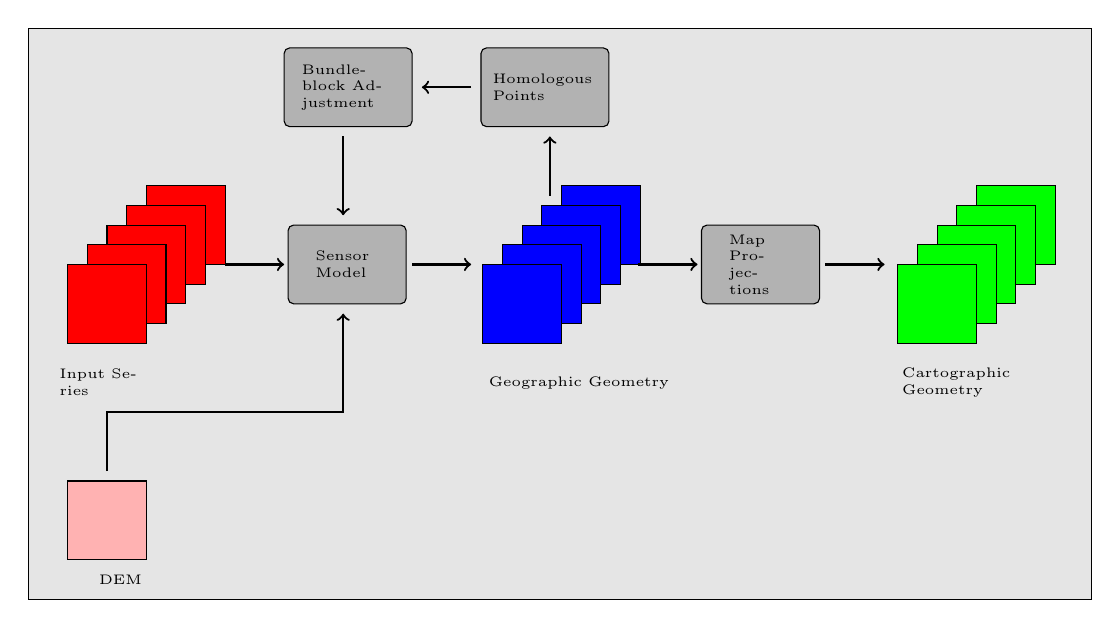
\begin{tikzpicture}[scale=0.25]
    \tiny
    \draw[fill=black!10] (-1,-12) rectangle (53,17);
     \foreach \x in {5,...,1}
       \draw[fill=red] (\x,\x) rectangle +(4,4);
     \node[fill=black!10, text width= 1.2cm] (InputSeries) at
       (3,-1) {Input Series};

     \draw[->,thick] (9,5) --  +(3,0);

     \draw[fill=black!30,rounded corners=2pt] (12.2,3) rectangle +(6,4);
     \node[text width= 0.7cm] (SensorModel) at (15,5) {Sensor Model};

     \draw[fill=red!30] (1,-10) rectangle +(4,4);
     \node[fill=black!10, text width= 1.2cm] (DEM) at
       (5,-11) {DEM};

     \draw[->,thick] (3,-5.5) --  ++(0,3) -- ++(12,0) -- ++(0,5);

     \draw[->,thick] (18.5,5) --  +(3,0);

     \foreach \x in {5,...,1}
       \draw[fill=blue,xshift=600pt] (\x,\x) rectangle +(4,4);
     \node[fill=black!10, text width= 2.8cm] (GeographicGeometry) at
       (28,-1) {Geographic Geometry};



       \draw[->,thick] (25.5,8.5) --  +(0,3);

     \draw[fill=black!30,rounded corners=2pt] (22,12) rectangle +(6.5,4);
     \node[text width= 0.7cm] (HomPoExtr) at (24,14) {Homologous
     Points};

     \draw[->,thick] (21.5,14) --  +(-2.5,0);

     \draw[fill=black!30,rounded corners=2pt] (12,12) rectangle +(6.5,4);
     \node[text width= 1.3cm] (BBAdj) at (15.5,14) {Bundle-block
     Adjustment};

     \draw[->,thick] (15,11.5) --  +(0,-4);


      \draw[->,thick] (30,5) --  +(3,0);

     \draw[fill=black!30,rounded corners=2pt] (33.2,3) rectangle +(6,4);
     \node[text width= 0.7cm] (MapProjection) at (36,5) {Map Projections};



     \draw[->,thick] (39.5,5) --  +(3,0);

     \foreach \x in {5,...,1}
       \draw[fill=green,xshift=1200pt] (\x,\x) rectangle +(4,4);
     \node[fill=black!10, text width= 1.8cm] (CartographicGeometry) at
       (47,-1) {Cartographic Geometry};

     %\draw[->,thick] (36,2) --  ++(0,-10) -- ++(-30,0);

  \end{tikzpicture}
  \itkcaption[Image Ortho-registration Procedure]{Image Ortho-registration Procedure.}
\label{fig:ImageOrtho-registrationProcedure}
\end{figure}

This chapter introduces the functionnalities available in OTB for
image ortho-registration. We define ortho-registration as the
procedure allowing to transform an image in sensor geometry to a
geographic or cartographic projection.\\

Figure \ref{fig:ImageOrtho-registrationProcedure} shows a synoptic
view of the different steps involved in a classical ortho-registration
processing chain able to deal with image series. These steps are the following:
\begin{itemize}
  \item Sensor modelling: the geometric sensor model allows to convert
  image coordinates (line, column) into geographic coordinates
  (latitude, longitude); a rigorous modelling needs a digital
  elevation model (DEM) in order to take into account the terrain
  topography.
  \item Bundle-block adjustment: in the case of image series, the
  geometric models and their parameters can be refined by using
  homologous points between the images. This is an optional step and
  not currently implemented in OTB.
  \item Map projection: this step allows to go from geographic
  coordinates to some specific cartographic projection as Lambert,
  Mercator or UTM.
\end{itemize}


\section{Sensor Models}
\ifitkFullVersion
\label{sec:SensorModels}
\fi

A sensor model is a set of equations giving the relationship between
image pixel $(l,c)$ coordinates and ground $(X,Y)$ coordinates for every
pixel in the image. Typically, the ground coordinates are given in a
geographic projection (latitude, longitude). The sensor model
can be expressed either from image to ground -- forward model -- or
from ground to image -- inverse model. This can be written as follows:

\begin{displaymath}
  \begin{array}{cc}
    Forward & \\
    X = f_x(l,c,h,\vec\theta) & Y = f_y(l,c,h,\vec\theta)\\
     & \\
    Inverse & \\
    l = g_l(X,Y,h,\vec\theta) & c = g_c(X,Y,h,\vec\theta)
  \end{array}
\end{displaymath}

Where $\vec\theta$ is the set of parameters which describe the sensor
and the acquisition geometry (platform altitude, viewing angle, focal
length for optical sensors, doppler centroid for SAR images, etc.).\\

In OTB, sensor models are implemented as \doxygen{itk}{Transform}s
(see section \ref{sec:Transforms} for details), which is the
appropriate way to express coordinate changes. The base class for
sensor models is \doxygen{otb}{SensorModelBase} from which the classes
\doxygen{otb}{InverseSensorModel} and
\doxygen{otb}{ForwardSensorModel} inherit.\\

As one may note from the model equations, the height of the ground, $h$,
must be known. Usually, it means that a Digital Elevation Model,
DEM, will be used.\\


\subsection{Types of Sensor Models}
\label{sec:TypesofSensorModels}
There exists two main types of sensor models. On one hand, we have the
so-called {\em physical models}, which are rigorous, complex,
eventually highly non-linear equations of the sensor geometry. As
such, they are difficult to inverse (obtain the inverse model from the
forward one and vice-versa). They have the significant advantage of having
parameters with physical meaning (angles, distances, etc.). They are
specific of each sensor, which means that a library of models is
required in the software. A library which has to be updated every time a new
sensor is available.\\

On the other hand, we have general analytical models, which
approximate the physical models. These models can take the form of
polynomials or ratios of polynomials, the so-called rational
polynomial functions or Rational Polynomial Coefficients, RPC, also
known as {\em Rapid Positioning Capability}.
Since they are approximations, they are less accurate than the
physical models. However, the achieved accuracy is usually high: in
the case of Pl\'eiades, RPC models have errors lower than 0.02 pixels
with respect to the physical model. Since these models have a standard
form they are easier to use and implement. However, they have the
drawback of having parameters (coefficients, actually) without
physical meaning.\\

OTB, through the use of the OSSIM library --
\url{http://www.ossim.org} -- offers models for most of current
sensors either through a physical or an analytical approach. This is
transparent for the user, since the geometrical model for a given
image is instantiated using the information stored in its meta-data. The 
search for a sensor model is not straightforward. It is done in several steps :
\begin{enumerate}
  \item Load an external \code{.geom} file specified through extended filenames
(if present)
  \item Load the \code{.geom} file attached with the input image (if present).
They share the same name, without extension.
  \item Search in the OSSIM plugin factory for a suitable model 
(\code{ossimplugins::ossimPluginProjectionFactory}). For instance, this
factory contains Pl\'eiades and TerraSar sensor models.
  \item If no model was found, search in the OSSIM projection factory 
(\code{ossimProjectionFactoryRegistry}). For instance this factory contains
Spot5, Landsat and Quickbird sensor models.
  \item If no model was found, search any RPC tags in the input image. When the
tags are present, an \code{ossimRpcModel} is created.
  \item If still no model was found, search for a valid sensor model in other
files attached to the current dataset. For instance, with a Sentinel-1 SAFE XML
product, it will inspect underlying \code{.tiff} files. With a VRT dataset, it
will inspect the files referenced by the VRT.
\end{enumerate}

Note that the \code{.geom} metadata file can store any sensor model recognized
by OSSIM.

\subsection{Using Sensor Models}
\label{sec:UsingSensorModels}

The transformation of an image in sensor geometry to geographic
geometry can be done using the following steps.
  \begin{enumerate}
    \item Read image meta-data and instantiate the model with the
    given parameters.
  \item Define the ROI in ground coordinates (this is your output
  pixel array)
  \item Iterate through the pixels of coordinates $(X,Y)$:
    \begin{enumerate}
      \item Get $h$ from the DEM
      \item Compute $(c,l) = G(X,Y,h,\vec\theta)$
      \item Interpolate pixel values if $(c,l)$ are not grid coordinates.
    \end{enumerate}
  \end{enumerate}

Actually, in OTB, you don't have to manually instantiate the sensor
model which is appropriate to your image. That is, you don't have to
manually choose a SPOT5 or a Quickbird sensor model. This task is
automatically performed by the \doxygen{otb}{ImageFileReader} class in
a similar way as the image format recognition is done. The appropriate
sensor model will then be included in the image meta-data, so you can
access it when needed.

\ifitkFullVersion
\input{SensorModelExample.tex}
\fi

\subsection{Evaluating Sensor Model}
\label{sec:EvaluatingSensorModels}

If no appropriate sensor model is available in the image meta-data,
OTB offers the possibility to estimate a sensor model from the image.

\input{EstimateRPCSensorModelExample.tex}


\subsection{Limits of the Approach}
\label{LimitsoftheApproach}

As you may understand by now, accurate geo-referencing needs accurate
DEM and also accurate sensor models and parameters. In the case where
we have several images acquired over the same area by different
sensors or different geometric configurations, geo-referencing (geographical coordinates) or ortho-rectification
(cartographic coordinates) is not usually enough. Indeed, when working
with image series we usually want to compare them (fusion, change
detection, etc.) at the pixel level.\\

Since common DEM and sensor parameters do not allow for such an
accuracy, we have to use clever strategies to improve the
co-registration of the images. The classical one consists in refining
the sensor parameters by taking homologous points between the images
to co-register. This is called bundle block adjustment and will be
implemented in coming versions of OTB.

Even if the model parameters are refined, errors due to DEM accuracy
can not be eliminated. In this case, image to image registration can
be applied. These approaches are presented in chapters
\ref{chap:ImageRegistration} and \ref{sec:DisparityMapEstimation}.

%% \section{Bundle-block adjustment}
%% Problem position
%%   \begin{itemize}
%%     \item The image series is geo-referenced (using the available DEM,
%%     and the prior sensor parameters).
%%     \item We assume that homologous points (GCPs, etc.) can be easily
%%     obtained from the geo-referenced series : $HP_i = (X_i,Y_i,h_i)$
%%     \item For each image, and each point, we can write:
%%     $(l_{ij},c_{ij}) = G_j(X_i,Y_i,h_i,\vec\theta_j)$
%%   \end{itemize}

%% \begin{tikzpicture}[scale=0.15]
%% \draw[fill=yellow!20] (-5.5,-15.5) rectangle (5.5,-5.5);
%%     \draw[step=0.5, gray, very thin] (-5.5,-15.5) grid (5.5,-5.5);

%%     \draw[fill=green!20,rotate=10] (-15.5,0.5) rectangle (-5.5,10.5);
%%     \draw[step=0.5, gray, very thin,rotate=10] (-15.5,0.5) grid>
%%     (-5.5,10.5);

%%     \draw[fill=blue!20,rotate=-10] (5.5,0.5) rectangle (15.5,10.5);
%%     \draw[step=0.5, gray, very thin,rotate=-10] (5.5,0.5) grid
%%     (15.5,10.5);


%%     \draw[fill=red!70] (1,-11) circle (0.2);

%%     \draw (1,-11) .. controls +(30:1cm) and +(60:1cm) .. (-10,7);

%%     \draw[fill=red!70] (-10,7) circle (0.2);

%%     \node (eq1) at (-12.2,-4) {$\scriptstyle{G_1(X_i,Y_i,h_i,\vec\theta_1)}$};

%%     \draw (1,-11) .. controls +(-30:1cm) and +(-60:1cm) .. (10,7);

%%     \draw[fill=red!70] (10,7) circle (0.2);

%%     \node (eq2) at (7.2,-3) {$\scriptstyle{G_2(X_i,Y_i,h_i,\vec\theta_2)}$};

%% \end{tikzpicture}
%% \begin{itemize}
%%       \item Everything is known.
%% \end{itemize}



%% Model refinement
%%   \begin{itemize}
%%     \item If we define $\vec\theta_j^R = \vec\theta_j +
%%     \vec{\Delta\theta_j}$ as the refined parameters,
%%     $\vec{\Delta\theta_j}$ are the unknowns of the model refinement
%%     problem.
%%     \item We have much more equations than unknowns if enough HPs are
%%     found.
%%     \item We solve using non-linear least squares estimation.
%%       \begin{itemize}
%% 	\item The derivatives of the sensor model with respect to its
%% 	parameters are needed.
%%       \end{itemize}
%%   \end{itemize}


%% Homologous point extraction
%% From manual to automatic procedures
%% \begin{itemize}
%%   \item Manual extraction can be used for a few images and for a few
%%   points
%%   \item We are interested in many images (long time series) and many
%%   points (in order to reduce registration errors)
%%   \item Proposed procedure
%%     \begin{enumerate}
%%       \item Choose candidate points
%%       \item Define a similarity measure
%%       \item Optimize the measure
%%     \end{enumerate}
%% \end{itemize}

%% Salient points
%% Similarity measures


\section{Map Projections}
\ifitkFullVersion
\label{sec:MapProjections}
\fi

Map projections describe the link between geographic coordinates and
cartographic ones. So map projections allow to represent a 2-dimensional manifold of a
3-dimensional space (the Earth surface) in a 2-dimensional space (a
map which used to be a sheet of paper!). This geometrical
transformation doesn't have a unique solution, so over the cartography
history, every country or region in the world has been able to express
the belief of being the center of the universe. In other words, every
cartographic projection tries to minimize the distortions of the 3D to
2D transformation for a given point of the Earth surface\footnote{We
  proposed to optimize an OTB map projection for Toulouse, but we
  didn't get any help from OTB users.}.

In OTB the \doxygen{otb}{MapProjection} class is derived from the
\doxygen{itk}{Transform} class, so the coordinate transformation
points are overloaded with map projection equations. The
\doxygen{otb}{MapProjection} class is templated over the type of
cartographic projection, which is provided by the OSSIM library. In
order to hide the complexity of the approach, some type definitions
for the more common projections are given in the file
\code{otbMapProjections.h} file.

Sometimes, you don't know at compile time what map projection you will need in
your application. In this case, the \doxygen{otb}{GenericMapProjection}
allow you to set the map projection at run-time by passing the WKT identification
for the projection.

\input{MapProjectionExample.tex}

You will seldom use a map projection by itself, but rather in an
ortho-rectification framework. An example is given in the next section.




\section{Orthorectification with OTB}
\ifitkFullVersion
\label{sec:OrthorectificationwithOTB}
\fi
\input{OrthoRectificationExample.tex}

\section{Vector data projection manipulation}
\ifitkFullVersion
\label{sec:VectorDataProjection}
\fi
\input{VectorDataProjectionExample.tex}

\section{Geometries projection manipulation}
\ifitkFullVersion
\label{sec:GeometriesProjection}
\fi
\input{GeometriesProjectionExample.tex}

\section{Elevation management with OTB}
\input{DEMHandlerExample.tex}

\section{Vector data area extraction}
\ifitkFullVersion
\label{sec:VectorDataAreaExtraction}
\fi
\input{VectorDataExtractROIExample.tex}

\input{Radiometry.tex}
\input{Fusion.tex}
\chapter{Feature Extraction}

% \section{Introduction}

Under the term {\em Feature Extraction} we include several techniques
aiming to detect or extract information of low level of abstraction
from images. These {\em features} can be objects : points, lines,
etc. They can also be measures : moments, textures, etc.

\section{Textures}
\subsection{Haralick Descriptors}

This example illustrates the use of the \doxygen{otb}{ScalarImageToTexturesFilter},
which compute the standard Haralick's textural features~\cite{Haralick1973} presented in table~\ref{tab:haralickStandardFeatures},
where $\mu_t$ and $\sigma_t$ are the mean and standard deviation of the row
(or column, due to symmetry) sums, $ \mu =  $ (weighted pixel average)
$ = \sum_{i,j}i \cdot g(i, j) =\sum_{i,j}j \cdot g(i, j) $ due to matrix summetry, and
$ \sigma =  $ (weighted pixel variance) $ = \sum_{i,j}(i - \mu)^2 \cdot g(i, j) =\sum_{i,j}(j - \mu)^2 \cdot g(i, j)  $
due to matrix symmetry.

\begin{table}
\begin{center}
\begin{tabular}{|c|c|}
\hline
& \\
Energy & $ f_1 = \sum_{i,j}g(i, j)^2 $ \\
& \\
\hline
& \\
Entropy & $ f_2 = -\sum_{i,j}g(i, j) \log_2 g(i, j)$, or 0 if $g(i, j) = 0$ \\
& \\
\hline
& \\
Correlation & $ f_3 = \sum_{i,j}\frac{(i - \mu)(j - \mu)g(i, j)}{\sigma^2} $ \\
& \\
\hline
& \\
Difference Moment &  $f_4 = \sum_{i,j}\frac{1}{1 + (i - j)^2}g(i, j) $ \\
& \\
\hline
& \\
Inertia (a.k.a. Contrast) & $ f_5 = \sum_{i,j}(i - j)^2g(i, j) $ \\
& \\
\hline
& \\
Cluster Shade & $ f_6 = \sum_{i,j}((i - \mu) + (j - \mu))^3 g(i, j) $ \\
& \\
\hline
Cluster Prominence & $ f_7 = \sum_{i,j}((i - \mu) + (j - \mu))^4 g(i, j) $ \\
& \\
\hline
& \\
Haralick's Correlation & $ f_8 = \frac{\sum_{i,j}(i, j) g(i, j) -\mu_t^2}{\sigma_t^2} $ \\
& \\
\hline
\end{tabular}
\itkcaption[Haralick features]{Haralick features~\cite{Haralick1973} available in \doxygen{otb}{ScalarImageToTexturesFilter}}
\end{center}
\label{tab:haralickStandardFeatures}
\end{table}

More features are available in \doxygen{otb}{ScalarImageToAdvancedTexturesFilter}.
\relatedClasses
\begin{itemize}
\item \doxygen{otb}{ScalarImageToAdvancedTexturesFilter}
\item \doxygen{otb}{ScalarImageToPanTexTextureFilter}
\item \doxygen{otb}{GreyLevelCooccurrenceIndexedList}
\end{itemize}

\input{TextureExample}

\subsection{PanTex}
\input{PanTexExample}

\subsection{Structural Feature Set}
\input{SFSExample}

\section{Interest Points}
\subsection{Harris detector}
\input{HarrisExample}
\subsection{SIFT detector}
\label{sec:SIFTDetector}
% \input{SIFTFastExample}
\InputIfFileExists{SIFTFastExample.tex}{}{}
\subsection{SURF detector}
\input{SURFExample}

\section{Alignments}
\label{sec:Alignments}
\input{AlignmentsExample}
\section{Lines}
\label{sec:LineDetectors}

\subsection{Line Detection}
\label{sec:LineDetection}
\input{RatioLineDetectorExample}
\input{CorrelationLineDetectorExample}
\input{AsymmetricFusionOfLineDetectorExample}
\input{ParallelLineDetectionExample}


\subsection{Segment Extraction}
\label{sec:SegmentExtraction}
\subsubsection{Local Hough Transform}
\input{LocalHoughExample}
%\input{ExtractSegmentsByStepsExample}
%\input{ExtractSegmentsExample}

\subsubsection{Line Segment Detector}
\label{sec:LSD}
\input{LineSegmentDetectorExample}
\subsection{Right Angle Detector}
\label{sec:RightAngleDetector}
\input{RightAngleDetectionExample}


\section{Density Features}
An interesting approach to feature extraction consists in computing
the density of previously detected features as simple edges or
interest points.
\subsection{Edge Density}
\input{EdgeDensityExample}
\subsection{SIFT Density}
\InputIfFileExists{SIFTDensityExample.tex}{}{}

% \input{SIFTDensityExample}

\section{Geometric Moments}

\subsection{Complex Moments}
\label{sec:ComplexMoments}
The complex geometric moments are defined as:
\begin {equation}
c_{pq} = \int\limits_{-\infty}^{+\infty}\int\limits_{-\infty}^{+\infty}(x + iy)^p(x- iy)^qf(x,y)dxdy,
\label{2.2}
\end{equation}
where $x$ and $y$ are the coordinates of the image $f(x,y)$, $i$ is the
imaginary unit and
$p+q$ is the order of $c_{pq}$. The geometric moments are
particularly useful in the case of scale changes.

\subsubsection{Complex Moments for Images}
\input{ComplexMomentsImageFunctionExample}
\subsubsection{Complex Moments for Paths}
\input{ComplexMomentPathExample}

\subsection{Hu Moments}
\label{sec:HuMoments}
Using the algebraic moment theory, H. Ming-Kuel obtained a family of 7
invariants with respect to planar transformations called Hu invariants,
\cite{hu}. Those invariants can be seen as nonlinear combinations of
the complex moments. Hu invariants have
been very much used in object recognition during the last 30 years,
since they are invariant to rotation, scaling and translation. \cite{flusserinv} gives their expressions :

\begin{equation}
\begin{array}{cccc}
\phi_1 = c_{11};& \phi_2 = c_{20}c_{02};& \phi_3 = c_{30}c_{03};& \phi_4 = c_{21}c_{12};\\
\phi_5 = Re(c_{30}c_{12}^3);& \phi_6 = Re(c_{21}c_{12}^2);& \phi_7 = Im(c_{30}c_{12}^3).&\\
\end{array}
\end{equation}


\cite{dudani} have used these invariants for the recognition of
aircraft silhouettes. Flusser and Suk have used them for image
registration, \cite{flusser_2}.

\subsubsection{Hu Moments for Images}
\input{HuMomentsImageFunctionExample}
%\subsubsection{Hu Moments for Paths}
%\input{HuMomentPathExample}


\subsection{Flusser Moments}
\label{sec:FlusserMoments}
The Hu invariants have been modified and
improved by several authors. Flusser used these moments in order to
produce a new family of descriptors of order higher than 3,
\cite{flusserinv}. These descriptors are invariant to scale and
rotation. They have the following expressions:
\begin {equation}
\begin{array}{ccc}
\psi_1  = c_{11} = \phi_1; &  \psi_2  = c_{21}c_{12} = \phi_4; & \psi_3  = Re(c_{20}c_{12}^2) = \phi_6;\\
\psi_4  = Im(c_{20}c_{12}^2); & \psi_5  = Re(c_{30}c_{12}^3) = \phi_5;
& \psi_6  = Im(c_{30}c_{12}^3) = \phi_7.\\
\psi_7  = c_{22}; & \psi_8  = Re(c_{31}c_{12}^2); & \psi_9  = Im(c_{31}c_{12}~2);\\
\psi_{10} = Re(c_{40}c_{12}^4); & \psi_{11} = Im(c_{40}c_{12}^2). &\\

\end{array}
\end {equation}

\textbf{Examples}
\subsubsection{Flusser Moments for Images}
\input{FlusserMomentsImageFunctionExample}
%\subsubsection{Flusser Moments for Paths}
%\input{FlusserMomentPathExample}

\section{Road extraction}
\label{sec:RoadExtraction}

Road extraction is a critical feature for an efficient use of high resolution satellite images. There are many applications of road extraction: update of GIS database, reference for image registration, help for identification algorithms and rapid mapping for example.  Road network can be used to register an optical image with a map or an optical image with a radar image for example. Road network extraction can help for other algorithms: isolated building detection, bridge detection. In these cases, a rough extraction can be sufficient. In the context of response to crisis, a fast mapping is necessary: within 6~hours, infrastructures for the designated area are required. Within this timeframe, a manual extraction is inconceivable and an automatic help is necessary.

\subsection{Road extraction filter}

\input{ExtractRoadExample}

\subsection{Step by step road extraction}

\input{ExtractRoadByStepsExample}


% \section{Seam carving}
% \label{sec:SeamCarving}
%
% \input{SeamCarvingExample}
%
% \input{SeamCarvingOtherExample}

\section{Cloud Detection}
\input{CloudDetectionExample}

\input{MultiScaleAnalysis.tex}
\input{ImageSegmentation.tex}
\input{ImageSimulation.tex}
\input{DimensionReduction.tex}
\input{Classification.tex}
\input{ObjectBasedImageAnalysis.tex}
\input{ChangeDetection.tex}
\input{Hyperspectral.tex}
\input{Visualization.tex}

%%% \input{Applications.tex}



\part{Developer's guide}\label{part:developerguide}
\chapter{Iterators}
\label{sec:ImageIteratorsChapter}
\index{Iterators!image|(}
\index{Generic Programming}
This chapter introduces the \emph{image iterator}, an important generic
programming construct for image processing in ITK.  An iterator is a
generalization of the familiar C programming language pointer used to
reference data in memory.  ITK has a wide variety of image iterators, some of
which are highly specialized to simplify common image processing tasks.

The next section is a brief introduction that defines iterators in the context
of ITK.  Section \ref{sec:IteratorsInterface} describes the programming
interface common to most ITK image iterators.
Sections~\ref{sec:ImageIterators}--\ref{sec:NeighborhoodIterators} document
specific ITK iterator types and provide examples of how they are used.

\section{Introduction}
\label{sec:IteratorsIntroduction}
% Further define iterators in the context of generic programming.
\index{generic programming}
\index{Iterators!definition of}
Generic programming models define functionally independent components called
\emph{containers} and \emph{algorithms}.  Container objects store data and
algorithms operate on data.  To access data in containers, algorithms use a
third class of objects called \emph{iterators}.  An iterator is an
abstraction of a memory pointer.  Every container type must define its own
iterator type, but all iterators are written to provide a common interface so
that algorithm code can reference data in a generic way and maintain
functional independence from containers.

The iterator is so named because it is used for \emph{iterative}, sequential
access of container values.  Iterators appear in \code{for} and
\code{while} loop constructs, visiting each data point in turn.  
A C pointer, for example, is a type of iterator.  It can be moved
forward (incremented) and backward (decremented) through memory to
sequentially reference elements of an array. Many iterator implementations
have an interface similar to a C pointer.

\index{Iterators!advantages of}
In ITK we use iterators to write generic image processing code for images
instantiated with different combinations of pixel type, pixel
container type, and dimensionality.  Because ITK image iterators are
specifically designed to work with \emph{image} containers, their interface and
implementation is optimized for image processing tasks.  Using the ITK
iterators instead of accessing data directly through the
\doxygen{otb}{Image} interface has many advantages. Code is more
compact and often generalizes automatically to higher dimensions, algorithms
run much faster, and iterators simplify tasks such as multithreading and
neighborhood-based image processing.


\section{Programming Interface}
\label{sec:IteratorsInterface}

\index{Iterators!programming interface|(}
%Creating iterators
This section describes the standard ITK image iterator programming interface.
Some specialized image iterators may deviate from this standard or provide
additional methods.

\subsection{Creating Iterators}
\label{sec:CreatingIterators}

\index{Iterators!construction of}
All image iterators have at least one template parameter that is the image
type over which they iterate.  There is no restriction on the dimensionality
of the image or on the pixel type of the image.

\index{Iterators!and image regions}

An iterator constructor requires at least two arguments, a smart pointer to the
image to iterate across, and an image region. The image region, called the
\emph{iteration region}, is a rectilinear area in which iteration is
constrained.  The iteration region must be wholly contained within the image.
More specifically, a valid iteration region is any subregion of the image
within the current \code{BufferedRegion}.  See Section~\ref{sec:ImageSection}
for more information on image regions.

\index{Iterators!const}
There is a const and a non-const version of most ITK image iterators. A
non-const iterator cannot be instantiated on a non-const image pointer.
Const versions of iterators may read, but may not write pixel values.

Here is a simple example that defines and constructs a simple image iterator
for an \doxygen{otb}{Image}.

\small
\begin{verbatim}
  typedef otb::Image<float, 3> ImageType;
  typedef itk::ImageRegionConstIterator< ImageType > ConstIteratorType;
  typedef itk::ImageRegionIterator< ImageType > IteratorType;

  ImageType::Pointer image = SomeFilter->GetOutput();

  ConstIteratorType constIterator( image, image->GetRequestedRegion() );
  IteratorType iterator( image, image->GetRequestedRegion() );
\end{verbatim}
\normalsize

\subsection{Moving Iterators}
\label{sec:MovingIterators}
An iterator is described as \emph{walking} its iteration region.  At any
time, the iterator will reference, or ``point to'', one pixel location in the
N-dimensional (ND) image.  \emph{Forward iteration} goes from the beginning
of the iteration region to the end of the iteration region.  \emph{Reverse
iteration}, goes from just past the end of the region back to the beginning.
There are two corresponding starting positions for iterators, the
\emph{begin} position and the \emph{end} position.  An iterator can be moved
directly to either of these two positions using the following methods.

\index{forward iteration}
\index{reverse iteration}
\index{iteration region}
\index{Iterators!GoToBegin()}

\begin{itemize}
\item \textbf{\code{GoToBegin()}} Points the iterator to the first valid
data element in the region.

\index{Iterators!GoToEnd()}
\item \textbf{\code{GoToEnd()}} Points the iterator to \emph{one position past}
the last valid element in the region.
\end{itemize}

Note that the end position is not actually located within the iteration region.  This is
important to remember because attempting to dereference an iterator at its end
position will have undefined results.

%Moving iteators
ITK iterators are moved back and forth across their iterations using the 
decrement and increment operators.

\index{Iterators!operator++()}
\begin{itemize}
\item \textbf{\code{operator++()}} Increments the iterator one position in the
positive direction.  Only the prefix increment operator is defined for ITK image
iterators.

\index{Iterators!operator--}
\item \textbf{\code{operator--()}} Decrements the iterator one position in the
negative direction.  Only the prefix decrement operator is defined for ITK
image iterators. 
\end{itemize}

Figure~\ref{fig:WalkingIterator} illustrates typical iteration over
an image region.  Most iterators increment and decrement in the direction of
the fastest increasing image dimension, wrapping to the first position in the
next higher dimension at region boundaries.  In other words, an
iterator first moves across columns, then down rows, then from slice to slice,
and so on.

\begin{figure}
\centering
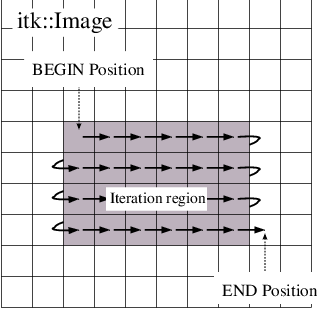
\includegraphics[width=0.4\textwidth]{IteratorFigure1.eps}
\itkcaption[ITK image iteration]{Normal path of an iterator through a 
2D image.  The iteration region is shown in a darker shade.  An arrow denotes
a single iterator step, the result of one \code{++} operation.}
\protect\label{fig:WalkingIterator}
\end{figure}

In addition to sequential iteration through the image, some iterators may define
random access operators.  Unlike the increment operators, random access
operators may not be optimized for speed and require some knowledge of the
dimensionality of the image and the extent of the iteration region to use properly.

\begin{itemize}
\index{Iterators!operator+=()}
\item \textbf{\code{operator+=( OffsetType )}} Moves the iterator to the pixel
position at the current index plus specified \doxygen{itk}{Offset}.

\index{Iterators!operator-=()}
\item \textbf{\code{operator-=( OffsetType )}} Moves the iterator to 
the pixel position at the current index minus specified Offset.

\index{Iterators!SetPosition()}
\item \textbf{\code{SetPosition( IndexType )}} Moves the iterator to the given
\doxygen{itk}{Index} position.
\end{itemize}

The \code{SetPosition()} method may be extremely slow for more complicated
iterator types. In general, it should only be used for setting a starting
iteration position, like you would use \code{GoToBegin()} or \code{GoToEnd()}.

Some iterators do not follow a predictable path through their
iteration regions and have no fixed beginning or ending pixel
locations.  A conditional iterator, for example, visits pixels only if
they have certain values or connectivities.  Random iterators,
increment and decrement to random locations and may even visit a given
pixel location more than once.

%Testing for location
An iterator can be queried to determine if it is at the end or the beginning of
its iteration region. 

\begin{itemize}
\index{Iterators!IsAtEnd()}
\item \textbf{\code{bool IsAtEnd()}} True if the iterator points to \emph{one
position past} the end of the iteration region.

\index{Iterators!IsAtBegin()}
\item \textbf{\code{bool IsAtBegin()}} True if the iterator points to the first
position in the iteration region.  The method is typically used to test for the
end of reverse iteration.

\end{itemize}

An iterator can also report its current image index position.

\begin{itemize}
\index{Iterators!GetIndex()}
\item \textbf{\code{IndexType GetIndex()}} Returns the Index
of the image pixel that the iterator currently points to.
\end{itemize}

% A note on bounds checking
\index{Iterators!and bounds checking}
For efficiency, most ITK image iterators do not perform bounds checking.  It is
possible to move an iterator outside of its valid iteration region.
Dereferencing an out-of-bounds iterator will produce undefined results.

\subsection{Accessing Data}
\label{sec:AccessingData}
ITK image iterators define two basic methods for reading and writing pixel
values.

\begin{itemize}
\index{Iterators!Get()}
\item \textbf{\code{PixelType Get()}} Returns the value of the pixel at the
iterator position.

\index{Iterators!Set()}
\item \textbf{\code{void Set( PixelType )}} Sets the value of the pixel at the
iterator position.  Not defined for const versions of iterators.
\end{itemize}

% Describe efficiency due to inlining for all cases
The \code{Get()} and \code{Set()} methods are inlined and optimized
for speed so that their use is equivalent to dereferencing the image
buffer directly.  There are a few common cases, however, where using
\code{Get()} and \code{Set()} do incur a penalty. Consider the
following code, which fetches, modifies, and then writes a value back
to the same pixel location.

\small
\begin{verbatim}
  it.Set( it.Get() + 1 );
\end{verbatim}
\normalsize

As written, this code requires one more memory dereference than is necessary.
Some iterators define a third data access method that avoids this penalty.

\begin{itemize}
\index{Iterators!Value()}
\item \textbf{\code{PixelType \& Value()}} Returns a reference to the pixel at
the iterator position.
\end{itemize}

The \code{Value()} method can be used as either an lval or an rval in an
expression.  It has all the properties of \code{operator*}.  The
\code{Value()} method makes it possible to rewrite our example code more
efficiently.

\small
\begin{verbatim}
  it.Value()++;
\end{verbatim}
\normalsize

Consider using the \code{Value()} method instead of \code{Get()} or
\code{Set()} when a call to \code{operator=} on a pixel is non-trivial, such as
when working with vector pixels, and operations are done in-place in the
image. The disadvantage of using \code{Value} is that it cannot support image
adapters (see Section~\ref{sec:ImageAdaptors} on
page~\pageref{sec:ImageAdaptors} for more information about image adaptors).

\subsection{Iteration Loops}
\label{sec:IterationExample}
% Now give a pseudo code example for putting all of this together.
Using the methods described in the previous sections, we can now write a simple
example to do pixel-wise operations on an image.  The following code calculates
the squares of all values in an input image and writes them to an output image.

\small
\begin{verbatim}
  ConstIteratorType in( inputImage,   inputImage->GetRequestedRegion() );
  IteratorType out( outputImage, inputImage->GetRequestedRegion() );

  for ( in.GoToBegin(), out.GoToBegin(); !in.IsAtEnd(); ++in, ++out )
    {
    out.Set( in.Get() * in.Get() );
    }
\end{verbatim}
\normalsize

\index{Iterators!and image regions}
Notice that both the input and output iterators are initialized over the same
region, the \code{RequestedRegion} of \code{inputImage}.  This is good
practice because it ensures that the output iterator walks exactly the same set
of pixel indices as the input iterator, but does not require that the output
and input be the same size. The only requirement is that the input image
must contain a region (a starting index and size) that matches the
\code{RequestedRegion} of the output image.

\index{reverse iteration}
Equivalent code can be written by iterating through the image in reverse.
The syntax is slightly more awkward because the \emph{end} of the
iteration region is not a valid position and we can only test whether the
iterator is strictly \emph{equal} to its beginning position.  It is often more
convenient to write reverse iteration in a \code{while} loop.

\small
\begin{verbatim}
  in.GoToEnd();
  out.GoToEnd();
  while ( ! in.IsAtBegin() )
    {
    --in;
    --out;
    out.Set( in.Get() * in.Get() );
    }
\end{verbatim}
\normalsize

%\begin{itemize}
%\item \textbf{\code{operator==}}
%\item \textbf{\code{operator<}} 
%\item \textbf{\code{operator<=}}
%\item \textbf{\code{operator>}}
%\item \textbf{\code{operator>=}}
%\end{itemize}

%operator +=, -=, etc

% SetIndex()

% operator <, operator >, etc.

\index{Iterators!programming interface|)}
\section{Image Iterators}
\label{sec:ImageIterators}
%Introduction and overview
This section describes iterators that walk rectilinear image regions and
reference a single pixel at a time.  The \doxygen{itk}{ImageRegionIterator} is the
most basic ITK image iterator and the first choice for most applications. The
rest of the iterators in this section are specializations of
ImageRegionIterator that are designed make common image processing
tasks more efficient or easier to implement.

% Each of the iterators has a const and non-const version

\subsection{ImageRegionIterator}
\index{itk::ImageRegionIterator|(}
\label{sec:itkImageRegionIterator}
\input{ImageRegionIterator.tex}
\index{itk::ImageRegionIterator|)}

\subsection{ImageRegionIteratorWithIndex}
\label{sec:itkImageRegionIteratorWithIndex}
\index{itk::ImageRegionIteratorWithIndex|(}
\input{ImageRegionIteratorWithIndex.tex}
\index{itk::ImageRegionIteratorWithIndex|)}

\subsection{ImageLinearIteratorWithIndex}
\label{sec:itkImageLinearIteratorWithIndex}
\index{itk::ImageLinearIteratorWithIndex|(}
\input{ImageLinearIteratorWithIndex.tex}
%\input{ImageLinearIteratorWithIndex2.tex}
\index{itk::ImageLinearIteratorWithIndex|)}

%% \subsection{ImageSliceIteratorWithIndex}
%% \label{sec:itkImageSliceIteratorWithIndex}
%% \index{itk::ImageSliceIteratorWithIndex|(}
%% \input{ImageSliceIteratorWithIndex.tex}
%% \index{itk::ImageSliceIteratorWithIndex|)}

%% \subsection{ImageRandomConstIteratorWithIndex}
%% \label{sec:itkImageRandomConstIteratorWithIndex}
%% \index{itk::Image\-Random\-Const\-Iterator\-With\-Index|(}
%% \input{ImageRandomConstIteratorWithIndex}
%% \index{itk::Image\-Random\-Const\-Iterator\-With\-Index|)}

%\section{Conditional Iterators}
%\index{Iterators!conditional|(}
%\label{sec:ConditionalIterators}
%This section describes iterators that walk only pixels in an image region whose
%values satisfy a specified condition.  The condition is usually based on some
%function of the image values, such as comparing to a threshold.  When the
%condition function returns \code{true} at a pixel location, the iterator
%includes that location in its path.  The biggest use of these iterators is for
%walking non-rectilinear regions of interest, such as might be defined by
%implicit geometric shape functions or connected component regions.

%./Common/itkConditionalConstIterator.h (BaseClass)
%./Common/itkConditionalIterator.h (BaseClass)
%./Common/itkFloodFilledFunctionConditionalConstIterator.h (BaseClass)
%./Common/itkFloodFilledFunctionConditionalIterator.h (BaseClass)

%[ here are all classes where these filters are used:
% ./BasicFilters/itkConfidenceConnectedImageFilter.hxx (ImageFunction)
% ./BasicFilters/itkConnectedThresholdImageFilter.hxx (ImageFunction)
% ./BasicFilters/itkIsolatedConnectedImageFilter.hxx (ImageFunction)
% ./BasicFilters/itkNeighborhoodConnectedImageFilter.hxx (ImageFunction)
%
% ./Common/itkBinaryBallStructuringElement.hxx (SpatialFunction)
% ./Common/itkBloxCoreAtomImage.hxx (SpatialFunction)
% ./BasicFilters/itkBloxBoundaryPointToCoreAtomImageFilter.hxx (SpatialFunction)
% ./BasicFilters/itkBloxBoundaryPointImageToBloxBoundaryProfileImageFilter.hxx (SpatialFunction)
%]

%\subsection{itk::FloodFilledImageFunctionConditionalIterator}
%\label{itk::FloodFilledImageFunctionConditionalIterator}
%\index{itk::FloodFilledImageFunctionConditionalIterator|(}
%./Common/itkFloodFilledImageFunctionConditionalConstIterator.h
%./Common/itkFloodFilledImageFunctionConditionalIterator.h
%\index{itk::FloodFilledImageFunctionConditionalIterator|)}

%\subsection{itk::FloodFilledSpatialFunctionConditionalIterator}
%\label{itk::FloodFilledSpatialFunctionConditionalIterator}
%\index{itk::FloodFilledSpatialFunctionConditionalIterator|(}
%./Common/itkFloodFilledSpatialFunctionConditionalConstIterator.h
%./Common/itkFloodFilledSpatialFunctionConditionalIterator.h
%\index{itk::FloodFilledImageFunctionConditionalIterator|)}
%\index{Iterators!conditional|)}

\section{Neighborhood Iterators}
\label{sec:NeighborhoodIterators}
\index{Iterators!neighborhood|(}
In ITK, a pixel neighborhood is loosely defined as a small set of pixels that
are locally adjacent to one another in an image.  The size and shape
of a neighborhood, as well the connectivity among pixels in a neighborhood,
may vary with the application.

Many image processing algorithms are neighborhood-based, that is, the result at
a pixel $i$ is computed from the values of pixels in the ND neighborhood of
$i$. Consider finite difference operations in 2D.  A derivative at pixel index
$i = (j, k)$, for example, is taken as a weighted difference of the values
at $(j+1, k)$ and $(j-1, k)$. Other common examples of neighborhood operations
include convolution filtering and image morphology.

This section describes a class of ITK image iterators that are designed for
working with pixel neighborhoods. An ITK neighborhood iterator walks an image
region just like a normal image iterator, but instead of only referencing a
single pixel at each step, it simultaneously points to the entire ND
neighborhood of pixels.  Extensions to the standard iterator interface provide
read and write access to all neighborhood pixels and information
such as the size, extent, and location of the neighborhood.

Neighborhood iterators use the same operators defined in
Section~\ref{sec:IteratorsInterface} and the same code constructs as normal
iterators for looping through an
image. Figure~\ref{fig:NeighborhoodIteratorFig1} shows a neighborhood iterator
moving through an iteration region.  This iterator defines a $3x3$ neighborhood
around each pixel that it visits. The \emph{center} of the neighborhood
iterator is always positioned over its current index and all other neighborhood
pixel indices are referenced as offsets from the center index.  The pixel
under the center of the neighborhood iterator and all pixels under the shaded
area, or \emph{extent}, of the iterator can be dereferenced.



\begin{figure}
\centering
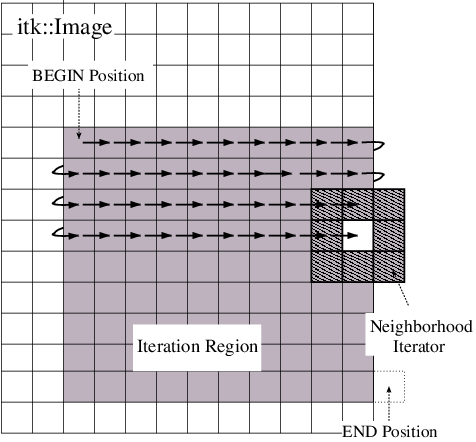
\includegraphics[width=0.6\textwidth]{NeighborhoodIteratorFig1.eps}
\itkcaption[Neighborhood iterator]{Path of a $3x3$ neighborhood
iterator through a 2D image region.  The extent of the neighborhood is
indicated by the hashing around the iterator position. Pixels that lie within
this extent are accessible through the iterator.  An arrow denotes a single
iterator step, the result of one \code{++} operation.}
\protect\label{fig:NeighborhoodIteratorFig1}
\end{figure}

\index{Neighborhood iterators!construction of}
\index{Neighborhood iterators!radius of}

In addition to the standard image pointer and iteration region
(Section~\ref{sec:IteratorsInterface}), neighborhood iterator constructors
require an argument that specifies the extent of the neighborhood to cover.
Neighborhood extent is symmetric across its center in each
axis and is given as an array of $N$ distances that are collectively called the
\emph{radius}. Each element $d$ of the radius, where $0 < d < N$ and
$N$ is the dimensionality of the neighborhood, gives the extent of the
neighborhood in pixels for dimension $N$.  The length of each face of the
resulting ND hypercube is $2d + 1$ pixels, a distance of $d$ on either side of
the single pixel at the neighbor center.
Figure~{\ref{fig:NeighborhoodIteratorFig2} shows the relationship between the
radius of the iterator and the size of the neighborhood for a variety of 2D
iterator shapes.

The radius of the neighborhood iterator is queried after construction
by calling the \code{GetRadius()} method.  Some other methods provide
some useful information about the iterator and its underlying image.

\begin{figure}
\centering
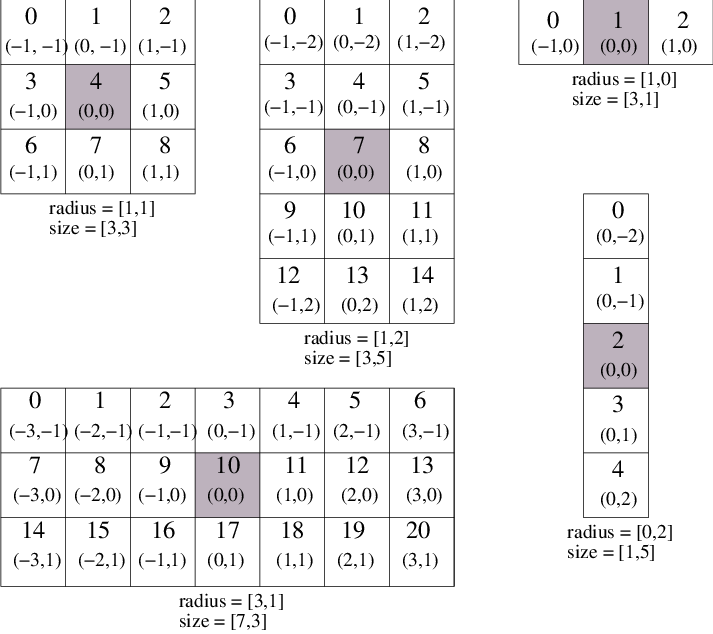
\includegraphics[width=0.9\textwidth]{NeighborhoodIteratorFig2.eps}
\itkcaption[Some possible neighborhood iterator shapes]{Several possible 2D
neighborhood iterator shapes are shown along with their radii and sizes.  A
neighborhood pixel can be dereferenced by its integer index (top) or its
offset from the center (bottom).  The center pixel of each iterator is
shaded.}
\protect\label{fig:NeighborhoodIteratorFig2}
\end{figure}

\begin{itemize}

\index{NeighborhoodIterator!GetRadius()}
\item \textbf{\code{SizeType GetRadius()}} Returns the ND radius of the
neighborhood as an \doxygen{itk}{Size}.

\index{NeighborhoodIterator!GetImagePointer()}
\item \textbf{\code{const ImageType *GetImagePointer()}} Returns the pointer to
the image referenced by the iterator.

\index{NeighborhoodIterator!Size()}
\item \textbf{\code{unsigned long Size()}} Returns the size in number of 
pixels of the neighborhood.

\end{itemize}

The neighborhood iterator interface extends the normal ITK iterator interface
for setting and getting pixel values.  One way to dereference pixels is to
think of the neighborhood as a linear array where each pixel has a unique
integer index. The index of a pixel in the array is determined by incrementing
from the upper-left-forward corner of the neighborhood along the fastest
increasing image dimension: first column, then row, then slice, and so on.  In
Figure~\ref{fig:NeighborhoodIteratorFig2}, the unique integer index is shown
at the top of each pixel.  The center pixel is always at position $n/2$, where
$n$ is the size of the array.

\begin{itemize}

\index{NeighborhoodIterator!GetPixel()}
\item \textbf{\code{PixelType GetPixel(const unsigned int i)}} Returns the 
value of the pixel at neighborhood position \code{i}.

\index{NeighborhoodIterator!SetPixel()}
\item \textbf{\code{void SetPixel(const unsigned int i, PixelType p)}} 
Sets the value of the pixel at position \code{i} to \code{p}.

\end{itemize}

Another way to think about a pixel location in a neighborhood is as an
ND offset from the neighborhood center.  The upper-left-forward corner
of a $3x3x3$ neighborhood, for example, can be described by offset
$(-1, -1, -1)$.  The bottom-right-back corner of the same neighborhood
is at offset $(1, 1, 1)$.  In
Figure~\ref{fig:NeighborhoodIteratorFig2}, the offset from center is
shown at the bottom of each neighborhood pixel.

\begin{itemize}

\index{NeighborhoodIterator!GetPixel()}
\item \textbf{\code{PixelType GetPixel(const OffsetType \&o)}} Get the value of
the pixel at the position offset \code{o} from the neighborhood center.

\index{NeighborhoodIterator!SetPixel()}
\item \textbf{\code{void SetPixel(const OffsetType \&o, PixelType p)}} Set
the value at the position offset \code{o} from the neighborhood center to
the value \code{p}.

\end{itemize}

The neighborhood iterators also provide a shorthand for setting and getting the
value at the center of the neighborhood.

\index{NeighborhoodIterators!}
\begin{itemize}

\index{NeighborhoodIterator!GetCenterPixel()}
\item \textbf{\code{PixelType GetCenterPixel()}} Gets the value at the center
of the neighborhood.

\index{NeighborhoodIterator!SetCenterPixel()}
\item \textbf{\code{void SetCenterPixel(PixelType p)}} Sets the value at the
center of the neighborhood to the value \code{p}

\end{itemize}

There is another shorthand for setting and getting values for pixels that
lie some integer distance from the neighborhood center along one of the image
axes.

\index{NeighborhoodIterators!}
\begin{itemize}

\index{NeighborhoodIterator!GetNext()}
\item \textbf{\code{PixelType GetNext(unsigned int d)}} Get the value
immediately adjacent to the neighborhood center in the positive direction along
the \code{d} axis.

\index{NeighborhoodIterator!SetNext()}
\item \textbf{\code{void SetNext(unsigned int d, PixelType p)}} Set the value
immediately adjacent to the neighborhood center in the positive direction along
the \code{d} axis to the value \code{p}.

\index{NeighborhoodIterator!GetPrevious()}
\item \textbf{\code{PixelType GetPrevious(unsigned int d)}} Get the value
immediately adjacent to the neighborhood center in the negative direction along
the \code{d} axis.

\index{NeighborhoodIterator!SetPrevious()}
\item \textbf{\code{void SetPrevious(unsigned int d, PixelType p)}}
Set the value immediately adjacent to the neighborhood center in the
negative direction along the \code{d} axis to the value \code{p}.

\item \textbf{\code{PixelType GetNext(unsigned int d, unsigned int
s)}} Get the value of the pixel located \code{s} pixels from the
neighborhood center in the positive direction along the \code{d} axis.

\item \textbf{\code{void SetNext(unsigned int d, unsigned int s, PixelType p)}}
Set the value of the pixel located \code{s} pixels from the neighborhood center
in the positive direction along the \code{d} axis to value \code{p}.

\item \textbf{\code{PixelType GetPrevious(unsigned int d, unsigned int
s)}} Get the value of the pixel located \code{s} pixels from the
neighborhood center in the positive direction along the \code{d} axis.
 
\item \textbf{\code{void SetPrevious(unsigned int d, unsigned int s,
PixelType p)}} Set the value of the pixel located \code{s} pixels from
the neighborhood center in the positive direction along the \code{d}
axis to value \code{p}.

\end{itemize}

It is also possible to extract or set all of the neighborhood values
from an iterator at once using a regular ITK neighborhood object.
This may be useful in algorithms that perform a particularly large
number of calculations in the neighborhood and would otherwise require
multiple dereferences of the same pixels.

\begin{itemize}

\index{NeighborhoodIterator!GetNeighborhood()}
\index{NeighborhoodIterator!SetNeighborhood()}
\item \textbf{\code{NeighborhoodType GetNeighborhood()}} Return a
\doxygen{itk}{Neighborhood} of the same size and shape as the neighborhood
iterator and contains all of the values at the iterator position.

\item \textbf{\code{void SetNeighborhood(NeighborhoodType \&N)}} Set all
of the values in the neighborhood at the iterator position to those contained
in Neighborhood \code{N}, which must be the same size and shape as the
iterator.

\end{itemize}

Several methods are defined to provide information about the neighborhood.

\index{NeighborhoodIterators!}
\begin{itemize}

\index{NeighborhoodIterator!GetIndex()}
\item \textbf{\code{IndexType GetIndex()}} Return the image
index of the center pixel of the neighborhood iterator.

\item \textbf{\code{IndexType GetIndex(OffsetType o)}} Return the
image index of the pixel at offset \code{o} from the neighborhood 
center.

\item \textbf{\code{IndexType GetIndex(unsigned int i)}} Return the
image index of the pixel at array position \code{i}.

\index{NeighborhoodIterator!GetOffset()}
\item \textbf{\code{OffsetType GetOffset(unsigned int i)}}  Return the offset
from the neighborhood center of the pixel at array position \code{i}.

\index{NeighborhoodIterator!GetNeighborhoodIndex()}
\item \textbf{\code{unsigned long GetNeighborhoodIndex(OffsetType o)}}
Return the array position of the pixel at offset \code{o} from the
neighborhood center.

\index{NeighborhoodIterator!GetSlice()}
\item \textbf{\code{std::slice GetSlice(unsigned int n)}} Return a
\code{std::slice} through the iterator neighborhood along axis \code{n}.

\end{itemize}

\index{Neighborhood iterators!boundary conditions}
\index{Neighborhood iterators!bounds checking}
A neighborhood-based calculation in a neighborhood close to an image
boundary may require data that falls outside the boundary.  The
iterator in Figure~\ref{fig:NeighborhoodIteratorFig1}, for example, is
centered on a boundary pixel such that three of its neighbors actually
do not exist in the image.  When the extent of a neighborhood falls
outside the image, pixel values for missing neighbors are supplied
according to a rule, usually chosen to satisfy the numerical
requirements of the algorithm.  A rule for supplying out-of-bounds
values is called a \emph{boundary condition}.
 
ITK neighborhood iterators automatically detect out-of-bounds dereferences and
will return values according to boundary conditions.  The boundary condition
type is specified by the second, optional template parameter of the iterator.
By default, neighborhood iterators use a Neumann condition where the first
derivative across the boundary is zero.  The Neumann rule simply returns the
closest in-bounds pixel value to the requested out-of-bounds location.  Several
other common boundary conditions can be found in the ITK toolkit.  They include
a periodic condition that returns the pixel value from the opposite side of the
data set, and is useful when working with periodic data such as Fourier
transforms, and a constant value condition that returns a set value $v$ for all
out-of-bounds pixel dereferences.  The constant value condition is equivalent
to padding the image with value $v$.

Bounds checking is a computationally expensive operation because it occurs each
time the iterator is incremented.  To increase efficiency, a neighborhood
iterator automatically disables bounds checking when it detects that it is
not necessary.  A user may also explicitly disable or enable bounds checking.
Most neighborhood based algorithms can minimize the need for bounds checking
through clever definition of iteration regions.  These techniques are explored
in Section~\ref{sec:NeighborhoodExample3}.

\begin{itemize}

\index{NeighborhoodIterator!NeedToUseBoundaryConditionOn()}
\item \textbf{\code{void NeedToUseBoundaryConditionOn()}} Explicitly turn
bounds checking on.  This method should be used with caution because
unnecessarily enabling bounds checking may result in a significant performance
decrease. In general you should allow the iterator to automatically determine
this setting.

\index{NeighborhoodIterator!NeedToUseBoundaryConditionOff()}
\item \textbf{\code{void NeedToUseBoundaryConditionOff()}} Explicitly disable
bounds checking. This method should be used with caution because disabling
bounds checking when it is needed will result in out-of-bounds reads and
undefined results.

\index{NeighborhoodIterator!OverrideBoundaryCondition()}
\item \textbf{\code{void OverrideBoundaryCondition(BoundaryConditionType *b)}} 
Overrides the templated boundary condition, using boundary condition
object \code{b} instead. Object \code{b} should not be deleted until
it has been released by the iterator.  This method can be used to
change iterator behavior at run-time.

\index{NeighborhoodIterator!ResetBoundaryCondition()}
\item \textbf{\code{void ResetBoundaryCondition()}} Discontinues the use of any
run-time specified boundary condition and returns to using the condition
specified in the template argument.

\index{NeighborhoodIterator!SetPixel()}
\item \textbf{\code{void SetPixel(unsigned int i, PixelType p, bool
status)}} Sets the value at neighborhood array position \code{i} to value
\code{p}.  If the position \code{i} is out-of-bounds, \code{status} is set to
\code{false}, otherwise \code{status} is set to \code{true}.
\end{itemize}

The following sections describe the two ITK neighborhood iterator classes,
\doxygen{itk}{NeighborhoodIterator} and \doxygen{itk}{ShapedNeighborhoodIterator}.
Each has a const and a non-const version.  The shaped iterator is a refinement
of the standard NeighborhoodIterator that supports an
arbitrarily-shaped (non-rectilinear) neighborhood.

\subsection{NeighborhoodIterator}
\label{sec:itkNeighborhoodIterator}

\index{NeighborhoodIterator!examples}
\index{Neighborhood iterators!examples}
The standard neighborhood iterator class in ITK is the
\doxygen{itk}{NeighborhoodIterator}.  Together with its \code{const} version,
\doxygen{itk}{ConstNeighborhoodIterator}, it implements the complete API
described above.  This section provides several examples to illustrate the use
of NeighborhoodIterator.

\index{edge detection}
\index{Sobel operator}
\subsubsection{Basic neighborhood techniques: edge detection}
\label{sec:NeighborhoodExample1}
\input{NeighborhoodIterators1.tex}

\index{convolution filtering}
\index{Sobel operator}
\subsubsection{Convolution filtering: Sobel operator}
\label{sec:NeighborhoodExample2}
\input{NeighborhoodIterators2.tex}

\subsubsection{Optimizing iteration speed}
\label{sec:NeighborhoodExample3}
\input{NeighborhoodIterators3.tex}

\index{Gaussian blurring}
\subsubsection{Separable convolution: Gaussian filtering}
\label{sec:NeighborhoodExample4}
\input{NeighborhoodIterators4.tex}

%% \subsubsection{Slicing the neighborhood}
%% \label{sec:NeighborhoodExample5}
%% \input{NeighborhoodIterators5.tex}

\subsubsection{Random access iteration}
\label{sec:NeighborhoodExample6}
\input{NeighborhoodIterators6.tex}

%./Common/itkConstNeighborhoodIterator.h
%./Common/itkNeighborhoodIterator.h

% Example1: Edge detection using ``hand-coded'' Sobel operator
% Example2: Sobel edge detection using convolution filtering and Sobel operator
% Example3: Improving boundary condition efficiency
% Example4: gaussian filtering, separable convolution
% Example5: Slicing the neighborhood: gaussian filtering, separable convolution
% Example6: Advanced Neighborhood Techniques: local minima, local maxima

\subsection{ShapedNeighborhoodIterator}
\label{sec:itkShapedNeighborhoodIterator}
\index{ShapedNeighborhoodIterator}
\index{Neighborhood iterators!shaped}
\index{Neighborhood iterators!as stencils}
This section describes a variation on the neighborhood iterator called a
\emph{shaped} neighborhood iterator.  A shaped neighborhood is defined like
a bit mask, or \emph{stencil}, with different offsets in the rectilinear
neighborhood of the normal neighborhood iterator turned off or on to create a
pattern.  Inactive positions (those not in the stencil) are not updated during
iteration and their values cannot be read or written.  The shaped iterator is
implemented in the class \doxygen{itk}{ShapedNeighborhoodIterator}, which is a
subclass of
\doxygen{itk}{NeighborhoodIterator}.  A const version,
\doxygen{itk}{ConstShapedNeighborhoodIterator}, is also available.

\index{Neighborhood iterators!active neighbors}
\index{Neighborhood iterators!inactive neighbors}
Like a regular neighborhood iterator, a shaped neighborhood iterator must be
initialized with an ND radius object, but the radius of the neighborhood of a
shaped iterator only defines the set of \emph{possible} neighbors.  Any number
of possible neighbors can then be activated or deactivated.  The shaped
neighborhood iterator defines an API for activating neighbors.  When a neighbor
location, defined relative to the center of the neighborhood, is activated, it
is placed on the \emph{active list} and is then part of the stencil.  An
iterator can be ``reshaped'' at any time by adding or removing offsets from the
active list.

\begin{itemize}

\index{ShapedNeighborhoodIterator!ActivateOffset()}
\item \textbf{\code{void ActivateOffset(OffsetType \&o)}} Include the offset
\code{o} in the stencil of active neighborhood positions.  Offsets are relative
to the neighborhood center.

\index{ShapedNeighborhoodIterator!DeactivateOffset()}
\item \textbf{\code{void DeactivateOffset(OffsetType \&o)}} Remove the offset
\code{o} from the stencil of active neighborhood positions.  Offsets are
relative to the neighborhood center. 

\index{ShapedNeighborhoodIterator!ClearActiveList()}
\item \textbf{\code{void ClearActiveList()}} Deactivate all positions in the
iterator stencil by clearing the active list.

\index{ShapedNeighborhoodIterator!GetActiveIndexListSize()}
\item \textbf{\code{unsigned int GetActiveIndexListSize()}} Return the number
of pixel locations that are currently active in the shaped iterator stencil.

\end{itemize}

Because the neighborhood is less rigidly defined in the shaped iterator, the
set of pixel access methods is restricted.  Only the \code{GetPixel()} and
\code{SetPixel()} methods are available, and calling these methods on an 
inactive neighborhood offset will return undefined results.

For the common case of traversing all pixel offsets in a neighborhood, the
shaped iterator class provides an iterator through the active offsets in its
stencil.   This \emph{stencil iterator} can be incremented or decremented and
defines \code{Get()} and \code{Set()} for reading and writing the values in the
neighborhood.

\begin{itemize}
\index{ShapedNeighborhoodIterator!Iterator::Begin()}
\item \textbf{\code{ShapedNeighborhoodIterator::Iterator Begin()}} Return a
const or non-const iterator through the shaped iterator stencil that points to
the first valid location in the stencil.

\index{ShapedNeighborhoodIterator!Iterator::End()}
\item \textbf{\code{ShapedNeighborhoodIterator::Iterator End()}} Return a
const or non-const iterator through the shaped iterator stencil that points
\emph{one position past} the last valid location in the stencil.
\end{itemize}

The functionality and interface of the shaped neighborhood iterator is best
described by example.  We will use the ShapedNeighborhoodIterator to
implement some binary image morphology algorithms (see \cite{Gonzalez1993},
\cite{Castleman1996}, et al.).  The examples that follow implement erosion and
dilation.

\index{ShapedNeighborhoodIterator!examples of}
\subsubsection{Shaped neighborhoods: morphological operations}
\label{sec:ShapedNeighborhoodExample}
\input{ShapedNeighborhoodIterators1.tex}
\input{ShapedNeighborhoodIterators2.tex}

%./Common/itkConstShapedNeighborhoodIterator.h
%./Common/itkShapedNeighborhoodIterator.h

\index{Iterators!neighborhood|)}

% ADD A SECTION WITH TIPS, SUGGESTIONS ON USING ITERATORS?  EXTENDING ITERATORS?
% USING ITERATORS FOR MULTITHREADING EXAMPLE?
\index{Iterators!image|)}

\input{ImageAdaptors.tex}
\input{StreamingAndThreading.tex}
\chapter{How To Write A Filter}
\label{chapter:WriteAFilter}

This purpose of this chapter is help developers create their own
filter (process object).  This chapter is divided into four major
parts. An initial definition of terms is followed by an overview of
the filter creation process. Next, data streaming is discussed. The
way data is streamed in ITK must be understood in order to write
correct filters. Finally, a section on multithreading describes what
you must do in order to take advantage of shared memory parallel
processing.

\section{Terminology}
\label{sec:Terminology}

The following is some basic terminology for the discussion that follows.
Chapter \ref{chapter:SystemOverview} provides additional background
information.

\begin{itemize}
        \item The \textbf{data processing pipeline} is a directed graph of
        \textbf{process} and \textbf{data objects}. The pipeline inputs,
        operators on, and outputs data.
        \index{data processing pipeline}
        \index{process object}
        \index{data object}

        \item A \textbf{filter}, or \textbf{process object}, has one or more
        inputs, and one or more outputs.
        \index{filter}

        \item A \textbf{source}, or source process object, initiates the data
        processing pipeline, and has one or more outputs.
        \index{source}

        \item A \textbf{mapper}, or mapper process object, terminates the
        data processing pipeline. The mapper has one or more outputs, and may
        write data to disk, interface with a display system, or interface to
        any other system.
        \index{mapper}

        \item A \textbf{data object} represents and provides access to
        data. In ITK, the data object (ITK class \doxygen{itk}{DataObject}) is 
        typically of type \doxygen{otb}{Image} or \doxygen{itk}{Mesh}.
        \index{data object}

        \item A \textbf{region} (ITK class \doxygen{itk}{Region}) represents a 
        piece, or subset of the entire data set.
        \index{region}

        \item An \textbf{image region} (ITK class \doxygen{itk}{ImageRegion})
        represents a structured portion of data. ImageRegion is implemented
        using the \doxygen{itk}{Index} and \doxygen{itk}{Size} classes
        \index{image region}

        \item A \textbf{mesh region} (ITK class \doxygen{itk}{MeshRegion}) 
        represents an unstructured portion of data.
        \index{mesh region}

        \item The \textbf{LargestPossibleRegion} is the theoretical single,
        largest piece (region) that could represent the entire dataset. The
        LargestPossibleRegion is used in the system as the measure of the
        largest possible data size.
        \index{LargestPossibleRegion}

        \item The \textbf{BufferedRegion} is a contiguous block of memory
        that is less than or equal to in size to the
        LargestPossibleRegion. The buffered region is what has actually been
        allocated by a filter to hold its output.
        \index{BufferedRegion}

        \item The \textbf{RequestedRegion} is the piece of the dataset that a
        filter is required to produce. The RequestedRegion is less than or
        equal in size to the BufferedRegion. The RequestedRegion may differ
        in size from the BufferedRegion due to performance reasons. The
        RequestedRegion may be set by a user, or by an application that needs
        just a portion of the data.
        \index{RequestedRegion}

        \item The \textbf{modified time} (represented by ITK class
        \doxygen{itk}{TimeStamp}) is a monotonically increasing integer value that
        characterizes a point in time when an object was last modified.
        \index{modified time}

        \item \textbf{Downstream} is the direction of dataflow, from sources
        to mappers.
        \index{pipeline!downstream}

        \item \textbf{Upstream} is the opposite of downstream, from mappers
        to sources.
        \index{pipeline!upstream}

        \item The \textbf{pipeline modified time} for a particular data
        object is the maximum modified time of all upstream data objects and
        process objects.
        \index{pipeline!modified time}

        \item The term \textbf{information} refers to metadata that
        characterizes data. For example, index and dimensions are information
        characterizing an image region.
        \index{pipeline!information}
\end{itemize}

\section{Overview of Filter Creation}
\label{sec:OverviewFilterCreation}
\index{filter!overview of creation}

\itkpiccaption[Relationship between DataObjects and ProcessObjects]
{Relationship between DataObject and ProcessObject.
\label{fig:DataPipeLineOneConnection}}
\parpic(7cm,2.5cm)[r]{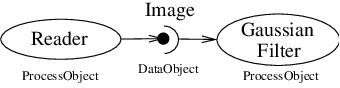
\includegraphics[width=6cm]{DataPipelineOneConnection.eps}}


Filters are defined with respect to the type of data they input (if
any), and the type of data they output (if any). The key to writing a
ITK filter is to identify the number and types of input and
output. Having done so, there are often superclasses that simplify
this task via class derivation. For example, most filters in ITK take
a single image as input, and produce a single image on output. The
superclass \doxygen{itk}{ImageToImageFilter} is a convenience class that
provide most of the functionality needed for such a filter.

Some common base classes for new filters include:

\begin{itemize}

  \item \code{ImageToImageFilter}: the most common filter base for
    segmentation algorithms.  Takes an image and produces a new image, by
    default of the same dimensions.  Override
    \code{GenerateOutputInformation} to produce a different size.

  \item \code{UnaryFunctorImageFilter}: used when defining a filter that
  applies a function to an image.

  \item \code{BinaryFunctorImageFilter}: used when defining a filter that
  applies an operation to two images.

  \item \code{ImageFunction}: a functor that can be applied to an image,
  evaluating $f(x) $ at each point in the image.

  \item \code{MeshToMeshFilter}: a filter that transforms meshes, such as
  tessellation, polygon reduction, and so on.

  \item \code{LightObject}: abstract base for filters that don't fit well
  anywhere else in the class hierarchy.  Also useful for ``calculator''
  filters; ie. a sink filter that takes an input and calculates a result
  which is retrieved using a \code{Get()} method.

\end{itemize}

Once the appropriate superclass is identified, the filter writer
implements the class defining the methods required by most all ITK
objects: \code{New()}, \code{PrintSelf()}, and protected constructor,
copy constructor, delete, and operator=, and so on. Also, don't forget
standard typedefs like \code{Self}, \code{Superclass}, \code{Pointer}, and
\code{ConstPointer}. Then the filter writer can focus on the most important
parts of the implementation: defining the API, data members, and other
implementation details of the algorithm. In particular, the filter writer
will have to implement either a \code{GenerateData()} (non-threaded) or
\code{ThreadedGenerateData()} method. (See Section~\ref{sec:MultiThreading}
for an overview of multi-threading in ITK.)

An important note: the GenerateData() method is required to allocate memory
for the output. The ThreadedGenerateData() method is not. In default
implementation (see \doxygen{itk}{ImageSource}, a superclass of
\doxygen{itk}{ImageToImageFilter})
\code{GenerateData()} allocates memory and then invokes
\code{ThreadedGenerateData()}.

One of the most important decisions that the developer must make is whether
the filter can stream data; that is, process just a portion of the input to
produce a portion of the output. Often superclass behavior works well: if the
filter processes the input using single pixel access, then the default
behavior is adequate. If not, then the user may have to a) find a more
specialized superclass to derive from, or b) override one or more methods
that control how the filter operates during pipeline execution. The next
section describes these methods.



\section{Streaming Large Data}
\label{sec:StreamingLargeData}
\index{pipeline!streaming large data}

The data associated with multi-dimensional images is large and becoming larger.
This trend is due to advances in scanning resolution, as well as increases in
computing capability. Any practical segmentation and registration software
system must address this fact in order to be useful in application. ITK
addresses this problem via its data streaming facility.

In ITK, streaming is the process of dividing data into pieces, or regions,
and then processing this data through the data pipeline. Recall that the
pipeline consists of process objects that generate data objects, connected
into a pipeline topology. The input to a process object is a data object
(unless the process initiates the pipeline and then it is a source process
object). These data objects in turn are consumed by other process objects,
and so on, until a directed graph of data flow is constructed. Eventually the
pipeline is terminated by one or more mappers, that may write data to
storage, or interface with a graphics or other system. This is illustrated in 
figures \ref{fig:DataPipeLineOneConnection} and \ref{fig:DataPipeLine}.

A significant benefit of this architecture is that the relatively complex
process of managing pipeline execution is designed into the system. This
means that keeping the pipeline up to date, executing only those portions of
the pipeline that have changed, multithreading execution, managing memory
allocation, and streaming is all built into the architecture. However, these
features do introduce complexity into the system, the bulk of which is seen
by class developers. The purpose of this chapter is to describe the pipeline
execution process in detail, with a focus on data streaming.


\subsection{Overview of Pipeline Execution}
\label{sec:OverviewPipelineExecution}
\index{pipeline!overview of execution}

The pipeline execution process performs several important functions.

\begin{figure}
  \par\centering
  \resizebox{5in}{!}{ 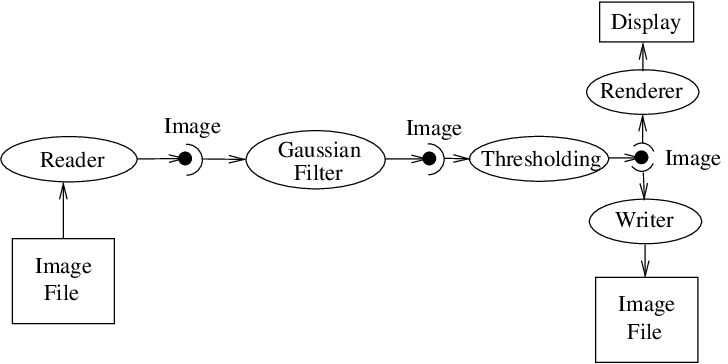
\includegraphics{DataPipeline.eps}} 
  \itkcaption[The Data Pipeline]{The Data Pipeline}
  \label{fig:DataPipeLine}
  \par
\end{figure}

\begin{enumerate}
        \item It determines which filters, in a pipeline of filters, need to
        execute. This prevents redundant execution and minimizes overall
        execution time.

        \item It initializes the (filter's) output data objects, preparing
        them for new data.  In addition, it determines how much memory each
        filter must allocate for its output, and allocates it.

        \item The execution process determines how much data a filter must
        process in order to produce an output of sufficient size for
        downstream filters; it also takes into account any limits on memory
        or special filter requirements. Other factors include the size of
        data processing kernels, that affect how much data input data 
        (extra padding) is required.

        \item It subdivides data into subpieces for multithreading. (Note
        that the division of data into subpieces is exactly same problem as
        dividing data into pieces for streaming; hence multithreading comes
        for free as part of the streaming architecture.)

        \item It may free (or release) output data if filters no longer need
        it to compute, and the user requests that data is to be
        released. (Note: a filter's output data object may be considered a
        ``cache''. If the cache is allowed to remain (\code{ReleaseDataFlagOff()}) 
        between pipeline execution, and the filter, or the input to the 
        filter, never changes, then process objects downstream of the filter 
        just reuse the filter's cache to re-execute.)
\end{enumerate}

To perform these functions, the execution process negotiates with the
filters that define the pipeline. Only each filter can know how much data is
required on input to produce a particular output. For example, a shrink
filter with a shrink factor of two requires an image twice as large (in terms
of its x-y dimensions) on input to produce a particular size output. An
image convolution filter would require extra input (boundary padding)
depending on the size of the convolution kernel. Some filters require the
entire input to produce an output (for example, a histogram), and have the
option of requesting the entire input. (In this case streaming does not work
unless the developer creates a filter that can request multiple pieces,
caching state between each piece to assemble the final output.)


\begin{figure}
  \par\centering
  \resizebox{5in}{!}{ 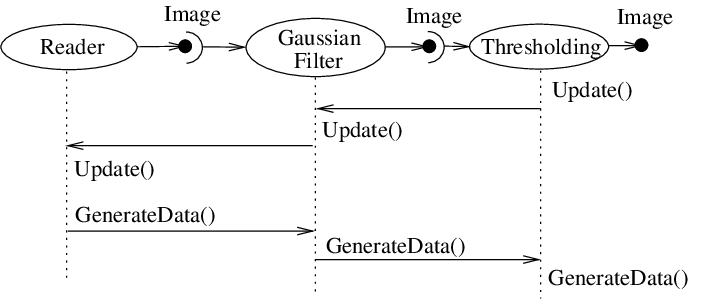
\includegraphics{DataPipelineUpdate.eps}} 
  \itkcaption[Sequence of the Data Pipeline updating mechanism]{Sequence of the
Data Pipeline updating mechanism}
  \label{fig:DataPipeLineUpdate}
  \par
\end{figure}


Ultimately the negotiation process is controlled by the request for data of a
particular size (i.e., region). It may be that the user asks to process a
region of interest within a large image, or that memory limitations result in
processing the data in several pieces. For example, an application may
compute the memory required by a pipeline, and then use
\doxygen{itk}{StreamingImageFilter} to break the data processing into several pieces.
The data request is propagated through the pipeline in the upstream
direction, and the negotiation process configures each filter to produce
output data of a particular size.

The secret to creating a streaming filter is to understand how this
negotiation process works, and how to override its default behavior by using
the appropriate virtual functions defined in \doxygen{itk}{ProcessObject}. The next
section describes the specifics of these methods, and when to override
them. Examples are provided along the way to illustrate concepts.


\subsection{Details of Pipeline Execution}
\label{sec:DetailsPipelineExecution}
\index{pipeline!execution details}

Typically pipeline execution is initiated when a process object
receives the \code{ProcessObject::Update()} method invocation. This
method is simply delegated to the output of the filter, invoking the
\code{DataObject::Update()} method. Note that this behavior is typical
of the interaction between ProcessObject and DataObject: a method
invoked on one is eventually delegated to the other. In this way the
data request from the pipeline is propagated upstream, initiating data
flow that returns downstream.

The \code{DataObject::Update()} method in turn invokes three other methods:

\begin{itemize}
        \item \code{DataObject::UpdateOutputInformation()}
        \item \code{DataObject::PropagateRequestedRegion()}
        \item \code{DataObject::UpdateOutputData()}
\end{itemize}

\subsubsection{UpdateOutputInformation()}
\label{sec:UpdateOutputInformation}
\index{pipeline!UpdateOutputInformation}

The \code{UpdateOutputInformation()} method determines the pipeline modified
time. It may set the RequestedRegion and the LargestPossibleRegion depending
on how the filters are configured. (The RequestedRegion is set to process all
the data, i.e., the LargestPossibleRegion, if it has not been set.) The
UpdateOutputInformation() propagates upstream through the entire pipeline and
terminates at the sources.

During \code{UpdateOutputInformation()}, filters have a chance to override the
\code{ProcessObject::GenerateOutputInformation()} method
(\code{GenerateOutputInformation()} is invoked by
\code{UpdateOutputInformation()}). The default behavior is for the
\code{GenerateOutputInformation()} to copy the metadata describing the input
to the output (via \code{DataObject::CopyInformation()}). Remember, information
is metadata describing the output, such as the origin, spacing,
and LargestPossibleRegion (i.e., largest possible size) of an image.

A good example of this behavior is \doxygen{itk}{ShrinkImageFilter}. This filter
takes an input image and shrinks it by some integral value. The result is that
the spacing and LargestPossibleRegion of the output will be different to that 
of the input. Thus, \code{GenerateOutputInformation()} is overloaded.

\subsubsection{PropagateRequestedRegion()}
\label{sec:PropagateRequestedRegion}
\index{pipeline!PropagateRequestedRegion}

The \code{PropagateRequestedRegion()} call propagates upstream to 
satisfy a data request. In typical application this data request is usually the
LargestPossibleRegion, but if streaming is necessary, or the user is
interested in updating just a portion of the data, the RequestedRegion may be
any valid region within the LargestPossibleRegion.

The function of \code{PropagateRequestedRegion()} is, given a request
for data (the amount is specified by RequestedRegion), propagate
upstream configuring the filter's input and output process object's to
the correct size. Eventually, this means configuring the
BufferedRegion, that is the amount of data actually allocated.

The reason for the buffered region is this: the output of a filter may be
consumed by more than one downstream filter. If these consumers each request
different amounts of input (say due to kernel requirements or other padding
needs), then the upstream, generating filter produces the data to satisfy
both consumers, that may mean it produces more data than one of the
consumers needs.

The \code{ProcessObject::PropagateRequestedRegion()} method invokes
three methods that the filter developer may choose to overload.

\begin{itemize}
        \item \code{EnlargeOutputRequestedRegion(DataObject *output)} gives the
        (filter) subclass a chance to indicate that it will provide more data
        than required for the output. This can happen, for example, when a
        source can only produce the whole output (i.e., the
        LargestPossibleRegion).

        \item \code{GenerateOutputRequestedRegion(DataObject *output)} gives 
        the subclass a chance to define how to set the requested regions for 
        each of its outputs, given this output's requested region.  The default
        implementation is to make all the output requested regions the same.
        A subclass may need to override this method if each output is a
        different resolution. This method is only overridden if a filter has
        multiple outputs.

        \item \code{GenerateInputRequestedRegion()} gives the subclass a 
        chance to
        request a larger requested region on the inputs. This is necessary
        when, for example, a filter requires more data at the ``internal''
        boundaries to produce the boundary values - due to kernel operations
        or other region boundary effects.
\end{itemize}

\doxygen{itk}{RGBGibbsPriorFilter} is an example of a filter that needs to
invoke \code{EnlargeOutputRequestedRegion()}. The designer of this
filter decided that the filter should operate on all the data. Note
that a subtle interplay between this method and
\code{GenerateInputRequestedRegion()} is occurring here. The default
behavior of \code{GenerateInputRequestedRegion()} (at least for
\doxygen{itk}{ImageToImageFilter}) is to set the input RequestedRegion to
the output's ReqestedRegion. Hence, by overriding the method
\code{EnlargeOutputRequestedRegion()} to set the output to the
LargestPossibleRegion, effectively sets the input to this filter to
the LargestPossibleRegion (and probably causing all upstream filters
to process their LargestPossibleRegion as well. This means that the
filter, and therefore the pipeline, does not stream. This could be
fixed by reimplementing the filter with the notion of streaming built
in to the algorithm.)

\doxygen{itk}{GradientMagnitudeImageFilter} is an example of a filter that needs to
invoke \code{GenerateInputRequestedRegion()}. It needs a larger input requested
region because a kernel is required to compute the gradient at a pixel. Hence
the input needs to be ``padded out'' so the filter has enough data to compute
the gradient at each output pixel.

\subsubsection{UpdateOutputData()}
\label{sec:UpdateOutputData}
\index{pipeline!UpdateOutputData}

\code{UpdateOutputData()} is the third and final method as a result of the
\code{Update()} method. The purpose of this method is to determine whether a
particular filter needs to execute in order to bring its output up to date. (A
filter executes when its \code{GenerateData()} method is invoked.) Filter
execution occurs when a) the filter is modified as a result of modifying an
instance variable; b) the input to the filter changes; c) the input data has
been released; or d) an invalid RequestedRegion was set previously and the
filter did not produce data. Filters execute in order in the downstream
direction.  Once a filter executes, all filters downstream of it must also
execute.

\code{DataObject::UpdateOutputData()} is delegated to the DataObject's source
(i.e., the ProcessObject that generated it) only if the DataObject needs to be
updated. A comparison of modified time, pipeline time, release data flag, and
valid requested region is made. If any one of these conditions indicate that
the data needs regeneration, then the source's
\code{ProcessObject::UpdateOutputData()} is invoked. These calls are made
recursively up the pipeline until a source filter object is encountered, or the
pipeline is determined to be up to date and valid. At this point, the recursion
unrolls, and the execution of the filter proceeds. (This means that the output
data is initialized, StartEvent is invoked, the filters \code{GenerateData()}
is called, EndEvent is invoked, and input data to this filter may be released,
if requested. In addition, this filter's InformationTime is updated to the
current time.)

The developer will never override \code{UpdateOutputData()}. The developer need
only write the \code{GenerateData()} method (non-threaded) or
\code{ThreadedGenerateData()} method. A discussion of threading follows in the
next section.


\section{Threaded Filter Execution}
\label{sec:ThreadedFilterExecution}
\index{pipeline!ThreadedFilterExecution}

Filters that can process data in pieces can typically multi-process
using the data parallel, shared memory implementation built into the
pipeline execution process. To create a multithreaded filter, simply
define and implement a \code{ThreadedGenerateData()} method. For
example, a \doxygen{itk}{ImageToImageFilter} would create the method:

\small
\begin{verbatim}
    void ThreadedGenerateData(const OutputImageRegionType& 
                              outputRegionForThread, itk::ThreadIdType threadId)
\end{verbatim}
\normalsize

The key to threading is to generate output for the output region given (as
the first parameter in the argument list above). In ITK, this is simple to do
because an output iterator can be created using the region provided. Hence
the output can be iterated over, accessing the corresponding input pixels as
necessary to compute the value of the output pixel.

Multi-threading requires caution when performing I/O (including using
\code{cout} or \code{cerr}) or invoking events. A safe practice is to allow 
only thread id zero to perform I/O or generate events. (The thread id is
passed as argument into \code{ThreadedGenerateData()}).  If more than one
thread tries to write to the same place at the same time, the program can
behave badly, and possibly even deadlock or crash.


\section{Filter Conventions}
\label{sec:FilterConventions}
\index{pipeline!filter conventions}

In order to fully participate in the ITK pipeline, filters are expected to
follow certain conventions, and provide certain interfaces.  This section
describes the minimum requirements for a filter to integrate into the ITK
framework.

The class declaration for a filter should include the macro
\code{ITK\_EXPORT}, so that on certain platforms an export declaration can be
included. 

A filter should define public types for the class itself (\code{Self}) and
its \code{Superclass}, and \code{const} and non-\code{const} smart pointers,
thus:

\begin{verbatim}
  typedef ExampleImageFilter                Self;
  typedef ImageToImageFilter<TImage,TImage> Superclass;
  typedef SmartPointer<Self>                Pointer;
  typedef SmartPointer<const Self>          ConstPointer;
\end{verbatim}

The \code{Pointer} type is particularly useful, as it is a smart pointer
that will be used by all client code to hold a reference-counted
instantiation of the filter. 

Once the above types have been defined, you can use the following
convenience macros, which permit your filter to participate in the object
factory mechanism, and to be created using the canonical \code{::New()}:

\begin{verbatim}
  /** Method for creation through the object factory. */
  itkNewMacro(Self);  

  /** Run-time type information (and related methods). */
  itkTypeMacro(ExampleImageFilter, ImageToImageFilter);
\end{verbatim}

The default constructor should be \code{protected}, and provide sensible
defaults (usually zero) for all parameters.  The copy constructor and
assignment operator should be declared \code{private} and not implemented,
to prevent instantiating the filter without the factory methods (above). 

Finally, the template implementation code (in the \code{.hxx} file) should
be included, bracketed by a test for manual instantiation, thus:

\begin{verbatim}
#ifndef ITK_MANUAL_INSTANTIATION
#include "itkExampleFilter.hxx"
#endif
\end{verbatim}

\subsection{Optional}
\label{sec:FilterPrinting}
\index{pipeline!printing a filter}

A filter can be printed to an \code{std::ostream} (such as \code{std::cout})
by implementing the following method:

\begin{verbatim}
  void PrintSelf( std::ostream& os, Indent indent ) const;
\end{verbatim}

\noindent and writing the name-value pairs of the filter parameters to the
supplied output stream.  This is particularly useful for debugging.

\subsection{Useful Macros}
\label{sec:UsefulMacros}
\index{pipeline!useful macros}

Many convenience macros are provided by ITK, to simplify filter coding. 
Some of these are described below:

\begin{description}
\item [itkStaticConstMacro] Declares a static variable of the given type,
  with the specified initial value. 
\item [itkGetMacro] Defines an accessor method for the specified scalar data
  member.  The convention is for data members to have a prefix of
  \code{m\_}. 
\item [itkSetMacro] Defines a mutator method for the specified scalar data
  member, of the supplied type.  This will automatically set the
  \code{Modified} flag, so the filter stage will be executed on the next
  \code{Update()}. 
\item [itkBooleanMacro] Defines a pair of \code{OnFlag} and \code{OffFlag}
  methods for a boolean variable \code{m\_Flag}.
\item [itkGetObjectMacro, itkSetObjectMacro] Defines an accessor and mutator
  for an ITK object.  The Get form returns a smart pointer to the object.
\end{description}

Much more useful information can be learned from browsing the source in
\code{Code/Common/itkMacro.h} and for the \doxygen{itk}{Object} and
\doxygen{itk}{LightObject} classes. 



%
% Section on how to write composite filters
%
\input{WriteACompositeFilter.tex}


%
% TODO: include useful tips from mailing list as flagged
%

\chapter{Persistent filters}
\label{chapter:PersistentFilters}

\section{Introduction}

As presented in chapter~\ref{sec:StreamingAndThreading}, OTB has two
main mechanisms to handle efficiently large data: streaming allows to
process image piece-wise, and multi-threading allows to process
concurrently several pieces of one streaming block. Using these
concepts, one can easily write pixel-wise or neighborhood-based
filters and insert them into a pipeline which will be scalable with
respect to the input image size.

Yet, sometimes we need to compute global features on the whole image. One
example is to determine image mean and variance of the input image in
order to produce a centered and reduced image. The operation of
centering and reducing each pixel is fully compliant with streaming and
threading, but one has to first estimate the mean and variance of the
image. This first step requires to walk the whole image once, and
traditional streaming and multi-threading based filter architecture is
of no help here. 

This is because there is a fundamental difference between these two
operations: one supports streaming, and the other needs to perform
streaming. In fact we would like to stream the whole image piece by
piece through some filter that will collect and keep mean and variance
cumulants, and then synthetize theses cumulants to compute the final
mean and variance once the full image as been streamed. Each
stream would also benefit from parallel processing. This is exactly
what persistent filters are for.

\section{Architecture}

There are two main objects in the persistent filters framework. The
first is the \doxygen{otb}{PersistentImageFilter}, the second is the
\doxygen{otb}{PersistentFilterStreamingDecorator}.

\subsection{The persistent filter class}

The \doxygen{otb}{PersistentImageFilter} class is a regular
\doxygen{itk}{ImageToImageFilter}, with two additional pure virtual
methods: the \verb?Synthetize()? and the \verb?Reset()? methods.

Imagine that the \verb?GenerateData()? or
\verb?ThreadedGenerateData()? progressively computes some global
feature of the whole image, using some member of the class to store
intermediate results. The \verb?Synthetize()? is an additional method
which is designed to be called one the whole image has been processed,
in order to compute the final results from the intermediate
results. The \verb?Reset()? method is designed to allow the reset of
the intermediate results members so as to start a fresh processing.

Any sub-class of the \doxygen{otb}{PersistentImageFilter} can be used
as a regular \doxygen{itk}{ImageToImageFilter} (provided that both
\verb?Synthetize()? and \verb?Reset()? have been implemented, but the
real interest of these filters is to be used with the streaming
decorator class presented in the next section.

\subsection{The streaming decorator class}

The \doxygen{otb}{PersistentFilterStreamingDecorator} is a class
designed to be templated with subclasses of the
\doxygen{otb}{PersistentImageFilter}. It provides the mechanism to
stream the whole image through the templated filter, using a third
class called \doxygen{otb}{StreamingImageVirtualWriter}. When the
\verb?Update()? method is called on a
\doxygen{otb}{PersistentFilterStreamingDecorator}, a pipeline
plugging the templated subclass of the
\doxygen{otb}{PersistentImageFilter} to an instance of
\doxygen{otb}{StreamingImageVirtualWriter} is created. The latter is
then updated, and acts like a regular
\doxygen{otb}{ImageFileWriter} but it does not actually write
anything to the disk : streaming pieces are requested and immediately
discarded. The \doxygen{otb}{PersistentFilterStreamingDecorator}
also calls the \verb?Reset()? method at the beginning and the
\verb?Synthetize()? method at the end of the streaming
process. Therefore, it packages the whole mechanism for the use of a
\doxygen{otb}{PersistentImageFilter}:
\begin{enumerate}
\item Call the \verb?Reset()? method on the filter so as to reset any temporary
  results members,
\item Stream the image piece-wise through the filter,
\item Call the \verb?Synthetize()? method on the filter so as to
  compute the final results.
\end{enumerate}

There are some methods that allows to tune the behavior of the
\doxygen{otb}{StreamingImageVirtualWriter}, allowing to change the
image splitting methods (tiles or strips) or the size of the streams
with respect to some target available amount of memory. Please see the
class documentation for details. The instance of the
\doxygen{otb}{StreamingImageVirtualWriter} can be retrieved from the
\doxygen{otb}{PersistentFilterStreamingDecorator} through the
\verb?GetStreamer()? method.

Though the internal filter of the
\doxygen{otb}{PersistentFilterStreamingDecorator} can be accessed
through the \verb?GetFilter()? method, the class is often derived to
package the streaming-decorated filter and wrap the parameters setters
and getters.

\section{An end-to-end example}

This is an end-to-end example to compute the mean over a full image,
using a streaming and threading-enabled filter. Please note that only
specific details are explained here. For more general information on
how to write a filter, please refer to
section~\ref{chapter:WriteAFilter}, page~\pageref{chapter:WriteAFilter}.

\subsection{First step: writing a persistent filter}

The first step is to write a persistent mean image filter. We need to
include the appropriate header :

\begin{cppcode}
#include "otbPersistentImageFilter.h"
\end{cppcode}

Then, we declare the class prototype as follows:

\begin{cppcode}
template<class TInputImage >
  class PersistentMeanImageFilter :
    public PersistentImageFilter<TInputImage, TInputImage>
\end{cppcode}

Since the output image will only be used for streaming purpose, we do
not need to declare different input and output template types.

In the \emph{private} section of the class, we will declare a member which
will be used to store temporary results, and a member which will be
used to store the final result.

\begin{cppcode}
private:
  // Temporary results container
  std::vector<PixelType> m_TemporarySums;

  // Final result member
  double m_Mean;
\end{cppcode}

Next, we will write the \verb?Reset()? method implementation in the
\emph{protected} section of the class. Proper allocation of the
temporary results container with respect to the number of threads is
handled here.


\begin{cppcode}
protected:
  virtual void Reset()
  {
  // Retrieve the number of threads
  unsigned int numberOfThreads = this->GetNumberOfThreads();

  // Reset the temporary results container
  m_TemporarySums = std::vector<PixelType>(numberOfThreads,
                                           itk::NumericTraits<PixelType>::Zero);

  // Reset the final result
  m_Mean = 0.;
  }
\end{cppcode}

Now, we need to write the \verb?ThreadedGenerateData()? methods (also
in the \emph{protected} section), were
temporary results will be computed for each piece of stream.

\begin{cppcode}
virtual void ThreadedGenerateData(const RegionType&
                                  outputRegionForThread, itk::ThreadIdType threadId)
{
// Enable progress reporting
itk::ProgressReporter(this,threadId,outputRegionForThread.GetNumberOfPixels());

// Retrieve the input pointer
InputImagePointer inputPtr = const_cast<TInputImage *>(this->GetInput());

// Declare an iterator on the region
itk::ImageRegionConstIteratorWithIndex<TInputImage> it(inputPtr,
outputRegionForThread);

// Walk the region of the image with the iterator
for (it.GoToBegin(); !it.IsAtEnd(); ++it, progress.CompletedPixel())
  {
  // Retrieve pixel value
  const PixelType& value = it.Get();

  // Update temporary results for the current thread
  m_TemporarySums[threadId]+= value;
}

\end{cppcode}

Last, we need to define the \verb?Synthetize()? method (still in the
\emph{protected} section), which will yield the final results:

\begin{cppcode}
virtual void Synthetize()
{
// For each thread
for(unsigned int threadId = 0; threadId <this->GetNumberOfThreads();++threadId)
  {
  // Update final result
  m_Mean+=m_TemporarySums[threadId];
} 

// Complete calculus by dividing by the total number of pixels:
unsigned int nbPixels =
this->GetInput()->GetLargestPossibleRegion().GetNumberOfPixels();

if(nbPixels!=0)
  {
  m_Mean/=nbPixels;
  }  
}
\end{cppcode}

\subsection{Second step: Decorating the filter and using it}

Now, to use the filter, one only has to decorate it with the
\doxygen{otb}{PersistentFilterStreamingDecorator}. First step is
to include the appropriate header:

\begin{cppcode}
#include "otbPersistentMeanImageFilter.h"
#include "otbPersistentFilterStreamingDecorator.h"
\end{cppcode}

Then, we decorate the filter with some typedefs:

\begin{cppcode}
typedef otb::PersistentMeanImageFilter<ImageType>
  PersitentMeanFilterType;
typedef otb::PersistentFilterStreamingDecorator
  < PersitentMeanFilterType> StreamingMeanFilterType;
\end{cppcode}

Now, the decorated filter can be used like any standard filter:

\begin{cppcode}
StreamingMeanFilterType::Pointer filter =
  StreamingMeanFilterType::New();

filter->SetInput(reader->GetOutput());
filter->Update();
\end{cppcode}

\subsection{Third step: one class to rule them all}

It is often convenient to avoid the few typedefs of the previous
section by deriving a new class from the decorated filter:

\begin{cppcode}
template<class TInputImage >
  class ITK_EXPORT StreamingMeanImageFilter :
    public PersistentFilterStreamingDecorator<
           PersistentImageFilter<TInputImage, TInputImage> >
\end{cppcode}

This also allows to redefine setters and getters for parameters,
avoiding to call the \verb?GetFilter()? method to set them.

\input{WriteAnApplication.tex}
\chapter{Adding New Modules}
\label{chapter:newModules}

This chapter is concerned with the creation of new modules.
The following sections give precise instructions about :
\begin{itemize}
	\item the organization of your directories
	\item the files you need to include
	\item what they must contain
	\item ...
\end{itemize}

\section{How to Write a Module}
\label{sec:writemodule}

There is a template of OTB remote module which help you  start developing you're
remote module: \href{https://gitlab.orfeo-toolbox.org/remote_modules/remote-module-template}{External Module Template}

Each module is made of different components, which are described in the following sections.

\section{The otb-module.cmake file}

This file is mandatory. It follows the CMake syntax, and has two purposes:

\begin{itemize}
       \item Declare dependencies to other modules,
       \item Provide a short description of the module purpose.
\end{itemize}

These purposes are fulfilled by a single CMake Macro call:

\begin{verbatim}
otb_module(TheModuleName DEPENDS OTBModule1 OTBModule2 ... OTBModuleN DESCRIPTION "A description string")
\end{verbatim}

\textbf{Note}: You can use the keyword TEST\textunderscore DEPENDS to declare module dependencies that only applies to the tests.

\section{The CMakeLists.txt file}

The CMakeLists.txt file is mandatory. It contains only a few things.
First, it declares a new CMake project with the name of the module.

\begin{verbatim}
project(TheModuleName)
\end{verbatim}

Second, if the module contain a library (see src folder section below), it initializes the TheModuleName\textunderscore LIBRARIES CMake variable (if your module only contains headers or template code, skip this line):

\begin{verbatim}
set(TheModuleName_LIBRARIES OTBTheModuleName)
\end{verbatim}

You can build your remote modules inside the OTB source tree by copying your
source inside the directory \textit{Module/Remote} or against an existing OTB
build tree (note that it does not work with an install version of OTB).

The configuration below will handle both cases and take care of all the CMake
plumbing of the module:

\begin{verbatim}
  if(NOT OTB_SOURCE_DIR)
    find_package(OTB REQUIRED)
    list(APPEND CMAKE_MODULE_PATH ${OTB_CMAKE_DIR})
    include(OTBModuleExternal)
  else()
    otb_module_impl()
  endif()
\end{verbatim}

The overall file should look like this:

\begin{verbatim}
cmake_minimum_required(VERSION 2.8.9)
project(TheModuleName)
set(ExternalTemplate_LIBRARIES OTBTheModuleName)

if(NOT OTB_SOURCE_DIR)
    find_package(OTB REQUIRED)
    list(APPEND CMAKE_MODULE_PATH ${OTB_CMAKE_DIR})
    include(OTBModuleExternal)
  else()
    otb_module_impl()
  endif()
\end{verbatim}

\section{The include folder}

The include folder will contain all your headers (*.h files) and template method boy files (*.hxx or *.hxx). It does not require any additional file (in particular, no CMakeLists.txt file is required).

\section{The src folder }

The src folder contains the internal implementation of your module :

\begin{itemize}
       \item  It typically contains cxx source files that will be compiled into a library.
       \item  It can contain header files for classes used only within the implementation files of your module. Any header file present in the src folder will not be installed, and will not be available to other modules depending on your module.
\end{itemize}

If your modules is made of template only code, you do not need a src folder at all.

If present, the src folder requires a CMakeLists.txt file.

The first part of the CMakeLists.txt file is classical, as it builds the library and links it:

\begin{verbatim}
set(OTBTheModuleName_SRC
    sourceFile1.cxx
    sourceFile2.cxx
    sourceFile3.cxx
    ...
    sourceFileN.cxx)

add_library(OTBTheModuleName ${OTBTheModuleName_SRC})

target_link_libraries(OTBTheModuleName ${OTBModule1_LIBRARIES} ${OTBModule2_LIBRARIES} ... ${OTBModuleN_LIBRARIES})
\end{verbatim}

\textbf{Notes}:

\begin{itemize}
       \item  Library name should match the one declared in the root CMakeLists.txt when setting CMake variable TheModuleName\textunderscore LIBRARIES,
       \item  Linked libraries should match the dependencies of your module declared in the root otb-module.cmake file.
\end{itemize}

The last line of CMake code takes care of installation instructions:
\begin{verbatim}
otb_module_target(TBTheModuleName)
\end{verbatim}

The overall CMakeLists.txt file should look like:

\begin{verbatim}
set(OTBTheModuleName_SRC
    sourceFile1.cxx
    sourceFile2.cxx
    sourceFile3.cxx
    ...
    sourceFileN.cxx)

add_library(OTBTheModuleName ${OTBTheModuleName_SRC})

target_link_libraries(OTBTheModuleName ${OTBModule1_LIBRARIES} ${OTBModule2_LIBRARIES} ... ${OTBModuleN_LIBRARIES})

otb_module_target(TBTheModuleName)
\end{verbatim}

\section{The app folder}

The app folder contains the code of applications shipped with your module. If your module has no application, you do not need the app folder.

\textbf{Notes}: If your module contains application (and an app folder), do not forget to add the ApplicationEngine in the dependencies listed in the otb-module.cmake file.

In addition to the applications source code, the app folder should contain a CMakeLists.txt file as follows.

For each application, a single call otb\textunderscore create\textunderscore application is required:

\begin{verbatim}
otb_create_application(
 NAME           TheModuleApplication1
 SOURCES        TheModuleApplication1.cxx
 LINK_LIBRARIES ${OTBModule1_LIBRARIES} ${OTBModule2_LIBRARIES} ... ${OTBModuleN_LIBRARIES})

\end{verbatim}

\section{The test folder}

This folder contains tests of the module. If your module has no test in it (which is not recommended, you do not need it).

The test folder should contain the source files of tests, as well as a CMakeLists.txt file. This file will contain the following.

First, indicate that this folder contains tests.

\begin{verbatim}
otb_module_test()
\end{verbatim}

Then, build the test driver:

\begin{verbatim}
set(OTBTheModuleNameTests
    testFile1.cxx
    testFile2.cxx
    ...
    testFileN.cxx)

add_executable(otbTheModuleNameTestDriver ${OTBTheModuleNameTests})

target_link_libraries(otbTheModuleNameTestDriver ${OTBTheModuleName-Test_LIBRARIES})

otb_module_target_label(otbTheModuleNameTestDriver)
\end{verbatim}

Finally, you can add your tests:

\begin{verbatim}
otb_add_test(NAME nameOfTheTest COMMAND otbTheModuleNameTestDriver
             --compare-image ${EPSILON_8} ... # baseline comparison if needed
             nameOfTheTestFunction
             testParameters)
\end{verbatim}

If your module contains one or more application in the app folder, you should
also write tests for them, in the test folder. Running an application test is
easily done with the helper macro otb\textunderscore test\textunderscore
application:

\begin{verbatim}
otb_test_application(NAME   nameofApplication1Test1
                      APP  TheModuleApplication1
                      OPTIONS -in1 ${INPUTDATA}/input1.tif
                              -in2 ${INPUTDATA}/input2.tif
                              -out ${TEMP}/nameofApplication1Test1_result.tif
                      VALID   --compare-image ${EPSILON_8}
                              ${BASELINE}/nameofApplication1Test1_result.tif
                              ${TEMP}/nameofApplication1Test1_result.tif)
\end{verbatim}

ToDo: Add instructions for test naming and input/baseline data inclusion.

You overall CMakeLists.txt file should look like:

\begin{verbatim}
otb_module_test()

set(OTBTheModuleNameTests
    testFile1.cxx
    testFile2.cxx
    ...
    testFileN.cxx)

add_executable(otbTheModuleNameTestDriver ${OTBTheModuleNameTests})

target_link_libraries(otbTheModuleNameTestDriver ${OTBTheModuleName-Test_LIBRARIES})

otb_module_target_label(otbTheModuleNameTestDriver)

otb_add_test(NAME nameOfTheTest COMMAND otbTheModuleNameTestDriver
             --compare-image ${EPSILON_8} ... # baseline comparison if needed
             nameOfTheTestFunction
             testParameters)
\end{verbatim}

\section{Including a remote module in OTB}
\begin{itemize}
       \item Local build of a remote module
\end{itemize}

Your remote module can be build inside the OTB source tree or outside as a
external CMake project with an existing OTB. Please note in that case
that you'll have to set OTB\textunderscore DIR CMake option.

If OTB\textunderscore DIR is an OTB build tree, there are two ways of compiling:
\begin{itemize}
  \item Build as a module, in which case build files will be written
    to the OTB build tree as other modules. Main benefit is that this
    will enrich the current OTB build with your new module, but you
    need to have write access to the build directory.
  \item Build as a standalone CMake project, in which case build files
    will remain in the module build folder. This build is fully
    independent from the build (or install) directory, but the module
    will not be recognized as an OTB module (still you will be able to
    use its binaries and libraries).
\end{itemize}

This behaviour is controlled by the OTB\textunderscore BUILD\textunderscore MODULE\textunderscore AS\textunderscore STANDALONE, which is OFF by default (hence first behaviour).

Note that when dealing with an installed OTB, only the second behaviour (build as standalone) is available.

Optionally, you can build your new remote module inside the OTB source tree by simply copy
the folder containing the module component to Modules/Remote, then run CMake
configuration. you should see a new CMake option named MODULE\textunderscore
TheModuleName. Simply turn this option to ON, and finish CMake
configuration. Your module will be built with the rest of the OTB project.

\begin{itemize}
       \item  Sharing your remote module
\end{itemize}

To make your remote module available to others when building OTB, you should
provide a CMake file named TheModuleName.remote.cmake file for inclusion in the
Modules/Remote folder in OTB source tree.

This file should contain the following:

\begin{verbatim}
#Contact: Author name <author email address>

otb_fetch_module(TheModuleName
  "A description of the module, to appear during CMake configuration step"
  GIT\textunderscore REPOSITORY http\textunderscore link\textunderscore to\textunderscore a\textunderscore git\textunderscore repository\textunderscore hosting\textunderscore the\textunderscore module
  GIT\textunderscore TAG the\textunderscore git\textunderscore revision\textunderscore to\textunderscore checkout
  )
\end{verbatim}
This file should be provided along with your remote module inclusion proposal email to the otb-developers list. Please refer to the contributors guidelines for more information (next section).

\input{Contribute.tex}

\part{Appendix}\label{part:appendix}

%Comment generation of wrapping documentation for release 3.2
\chapter{Wrappings to other languages}
\label{chap:wrappings}
%Set the code style to Java for the Wrapping

\input{Wrapping.tex}

\input{Contributors.tex}

\backmatter

%%%%%%%%%%%%%%%%%%%%%%%%%%%%%%%%%%%%%%%%%
%
%  Insert the bibliography using BibTeX
%
%%%%%%%%%%%%%%%%%%%%%%%%%%%%%%%%%%%%%%%%%

% \bibliographystyle{plain}
\bibliographystyle{abbrv}
\bibliography{\bibtexdatabasepath/Insight}


%%%%%%%%%%%%%%%%%%%%%%%%%%%%%%%%%%%%%%%%%
%
%  Insert the Index file
%
%%%%%%%%%%%%%%%%%%%%%%%%%%%%%%%%%%%%%%%%%

\InputIfFileExists{SoftwareGuide.ind}{}{}

%%\ifitkPrintedVersion
%%\cleardoublepage
%%% \input{MarketingMaterial.tex}
%%\fi

\end{document}



